% Options for packages loaded elsewhere
\PassOptionsToPackage{unicode}{hyperref}
\PassOptionsToPackage{hyphens}{url}
%
\documentclass[
]{book}
\usepackage{lmodern}
\usepackage{amssymb,amsmath}
\usepackage{ifxetex,ifluatex}
\ifnum 0\ifxetex 1\fi\ifluatex 1\fi=0 % if pdftex
  \usepackage[T1]{fontenc}
  \usepackage[utf8]{inputenc}
  \usepackage{textcomp} % provide euro and other symbols
\else % if luatex or xetex
  \usepackage{unicode-math}
  \defaultfontfeatures{Scale=MatchLowercase}
  \defaultfontfeatures[\rmfamily]{Ligatures=TeX,Scale=1}
\fi
% Use upquote if available, for straight quotes in verbatim environments
\IfFileExists{upquote.sty}{\usepackage{upquote}}{}
\IfFileExists{microtype.sty}{% use microtype if available
  \usepackage[]{microtype}
  \UseMicrotypeSet[protrusion]{basicmath} % disable protrusion for tt fonts
}{}
\makeatletter
\@ifundefined{KOMAClassName}{% if non-KOMA class
  \IfFileExists{parskip.sty}{%
    \usepackage{parskip}
  }{% else
    \setlength{\parindent}{0pt}
    \setlength{\parskip}{6pt plus 2pt minus 1pt}}
}{% if KOMA class
  \KOMAoptions{parskip=half}}
\makeatother
\usepackage{xcolor}
\IfFileExists{xurl.sty}{\usepackage{xurl}}{} % add URL line breaks if available
\IfFileExists{bookmark.sty}{\usepackage{bookmark}}{\usepackage{hyperref}}
\hypersetup{
  pdftitle={Treinamento Bookdown},
  pdfauthor={Robson Wilson Silva Pessoa, Ícaro Bernardes e Daniela Almeida},
  hidelinks,
  pdfcreator={LaTeX via pandoc}}
\urlstyle{same} % disable monospaced font for URLs
\usepackage{color}
\usepackage{fancyvrb}
\newcommand{\VerbBar}{|}
\newcommand{\VERB}{\Verb[commandchars=\\\{\}]}
\DefineVerbatimEnvironment{Highlighting}{Verbatim}{commandchars=\\\{\}}
% Add ',fontsize=\small' for more characters per line
\usepackage{framed}
\definecolor{shadecolor}{RGB}{248,248,248}
\newenvironment{Shaded}{\begin{snugshade}}{\end{snugshade}}
\newcommand{\AlertTok}[1]{\textcolor[rgb]{0.94,0.16,0.16}{#1}}
\newcommand{\AnnotationTok}[1]{\textcolor[rgb]{0.56,0.35,0.01}{\textbf{\textit{#1}}}}
\newcommand{\AttributeTok}[1]{\textcolor[rgb]{0.77,0.63,0.00}{#1}}
\newcommand{\BaseNTok}[1]{\textcolor[rgb]{0.00,0.00,0.81}{#1}}
\newcommand{\BuiltInTok}[1]{#1}
\newcommand{\CharTok}[1]{\textcolor[rgb]{0.31,0.60,0.02}{#1}}
\newcommand{\CommentTok}[1]{\textcolor[rgb]{0.56,0.35,0.01}{\textit{#1}}}
\newcommand{\CommentVarTok}[1]{\textcolor[rgb]{0.56,0.35,0.01}{\textbf{\textit{#1}}}}
\newcommand{\ConstantTok}[1]{\textcolor[rgb]{0.00,0.00,0.00}{#1}}
\newcommand{\ControlFlowTok}[1]{\textcolor[rgb]{0.13,0.29,0.53}{\textbf{#1}}}
\newcommand{\DataTypeTok}[1]{\textcolor[rgb]{0.13,0.29,0.53}{#1}}
\newcommand{\DecValTok}[1]{\textcolor[rgb]{0.00,0.00,0.81}{#1}}
\newcommand{\DocumentationTok}[1]{\textcolor[rgb]{0.56,0.35,0.01}{\textbf{\textit{#1}}}}
\newcommand{\ErrorTok}[1]{\textcolor[rgb]{0.64,0.00,0.00}{\textbf{#1}}}
\newcommand{\ExtensionTok}[1]{#1}
\newcommand{\FloatTok}[1]{\textcolor[rgb]{0.00,0.00,0.81}{#1}}
\newcommand{\FunctionTok}[1]{\textcolor[rgb]{0.00,0.00,0.00}{#1}}
\newcommand{\ImportTok}[1]{#1}
\newcommand{\InformationTok}[1]{\textcolor[rgb]{0.56,0.35,0.01}{\textbf{\textit{#1}}}}
\newcommand{\KeywordTok}[1]{\textcolor[rgb]{0.13,0.29,0.53}{\textbf{#1}}}
\newcommand{\NormalTok}[1]{#1}
\newcommand{\OperatorTok}[1]{\textcolor[rgb]{0.81,0.36,0.00}{\textbf{#1}}}
\newcommand{\OtherTok}[1]{\textcolor[rgb]{0.56,0.35,0.01}{#1}}
\newcommand{\PreprocessorTok}[1]{\textcolor[rgb]{0.56,0.35,0.01}{\textit{#1}}}
\newcommand{\RegionMarkerTok}[1]{#1}
\newcommand{\SpecialCharTok}[1]{\textcolor[rgb]{0.00,0.00,0.00}{#1}}
\newcommand{\SpecialStringTok}[1]{\textcolor[rgb]{0.31,0.60,0.02}{#1}}
\newcommand{\StringTok}[1]{\textcolor[rgb]{0.31,0.60,0.02}{#1}}
\newcommand{\VariableTok}[1]{\textcolor[rgb]{0.00,0.00,0.00}{#1}}
\newcommand{\VerbatimStringTok}[1]{\textcolor[rgb]{0.31,0.60,0.02}{#1}}
\newcommand{\WarningTok}[1]{\textcolor[rgb]{0.56,0.35,0.01}{\textbf{\textit{#1}}}}
\usepackage{longtable,booktabs}
% Correct order of tables after \paragraph or \subparagraph
\usepackage{etoolbox}
\makeatletter
\patchcmd\longtable{\par}{\if@noskipsec\mbox{}\fi\par}{}{}
\makeatother
% Allow footnotes in longtable head/foot
\IfFileExists{footnotehyper.sty}{\usepackage{footnotehyper}}{\usepackage{footnote}}
\makesavenoteenv{longtable}
\usepackage{graphicx,grffile}
\makeatletter
\def\maxwidth{\ifdim\Gin@nat@width>\linewidth\linewidth\else\Gin@nat@width\fi}
\def\maxheight{\ifdim\Gin@nat@height>\textheight\textheight\else\Gin@nat@height\fi}
\makeatother
% Scale images if necessary, so that they will not overflow the page
% margins by default, and it is still possible to overwrite the defaults
% using explicit options in \includegraphics[width, height, ...]{}
\setkeys{Gin}{width=\maxwidth,height=\maxheight,keepaspectratio}
% Set default figure placement to htbp
\makeatletter
\def\fps@figure{htbp}
\makeatother
\setlength{\emergencystretch}{3em} % prevent overfull lines
\providecommand{\tightlist}{%
  \setlength{\itemsep}{0pt}\setlength{\parskip}{0pt}}
\setcounter{secnumdepth}{5}
\usepackage{booktabs}
\usepackage[]{natbib}
\bibliographystyle{apalike}

\title{Treinamento Bookdown}
\author{Robson Wilson Silva Pessoa, Ícaro Bernardes e Daniela Almeida}
\date{2020-08-24}

\begin{document}
\maketitle

{
\setcounter{tocdepth}{1}
\tableofcontents
}
\begin{Shaded}
\begin{Highlighting}[]
\NormalTok{knitr}\OperatorTok{::}\NormalTok{opts_chunk}\OperatorTok{$}\KeywordTok{set}\NormalTok{(}\DataTypeTok{error =} \OtherTok{TRUE}\NormalTok{)}
\end{Highlighting}
\end{Shaded}

\hypertarget{pruxe9-requisitos}{%
\chapter{Pré-requisitos}\label{pruxe9-requisitos}}

Este documento foi elaborado a partir da estrutura mínima
obtida pelo \emph{template} do \emph{Bookdown} disponível no ambiente
do \emph{Rstudio}.

Este é um \emph{sample} da escrita em \textbf{Markdown}. É
possível utilizar qualquer recurso que suportado
pelo \emph{Markdown} do \emph{Pandoc}, como a
equação
\[f(x) = \frac{1}{\sigma\sqrt{2\pi}}\exp\left(-\frac{1}{2}\left(\frac{x-\mu}{\sigma}\right)^2\right)\].

A instalação do \textbf{bookdown} package pode instalado pelo CRAN ou Github. A seguir apresentamos uma sequência
de passos de instalação pelo modo gráfico. Se
você tem familiaridade pule a sequência de
figuras e instale utilizando os comandos na aba
\emph{Console}, caso contrário siga os seguintes passos:

\begin{enumerate}
\def\labelenumi{\arabic{enumi}.}
\tightlist
\item
  Primeiro é necessário abrir o Rstudio,
\end{enumerate}

\begin{figure}
\centering
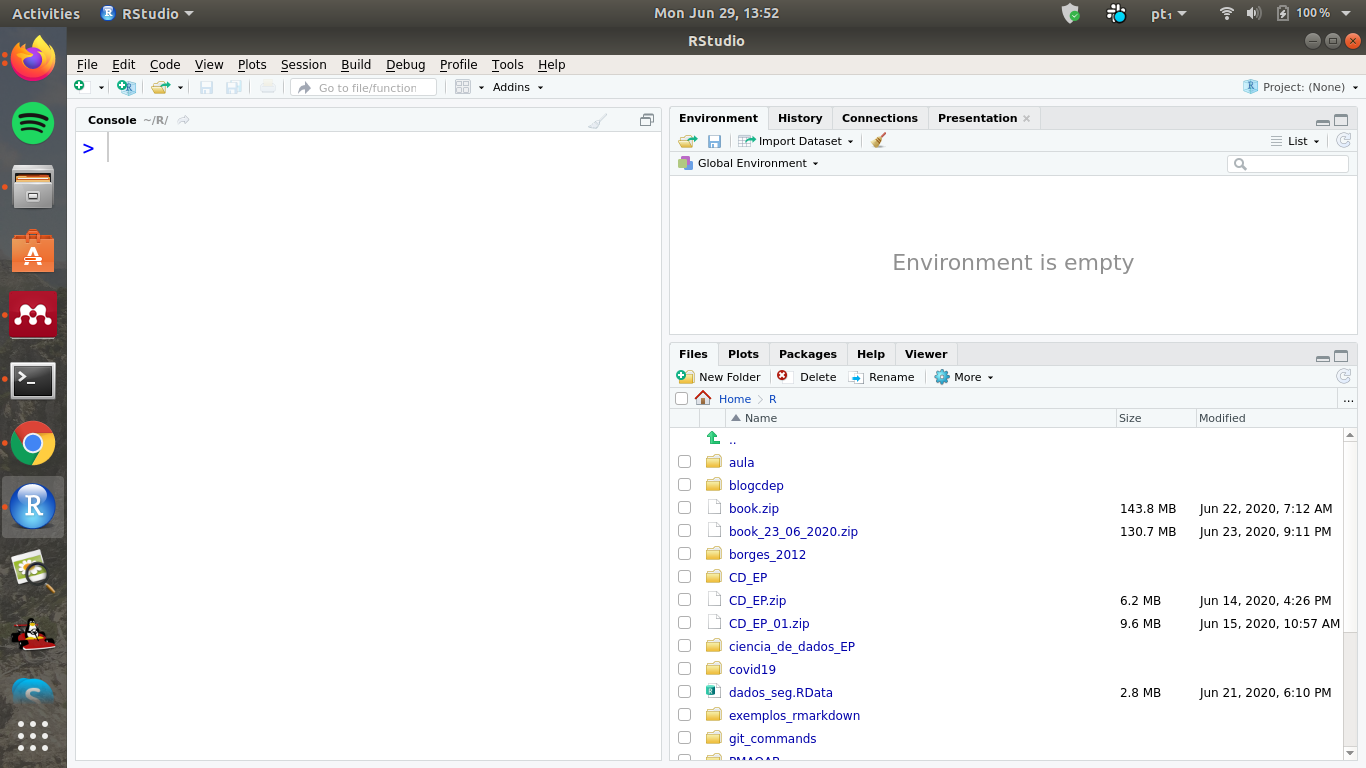
\includegraphics{fig/open_Rstudio.png}
\caption{Opção de instalação pelo modo gráfico}
\end{figure}

\begin{enumerate}
\def\labelenumi{\arabic{enumi}.}
\setcounter{enumi}{1}
\tightlist
\item
  Selecoine a aba de instalação \emph{Packages} e clique em \textbf{install},
\end{enumerate}

\begin{figure}
\centering
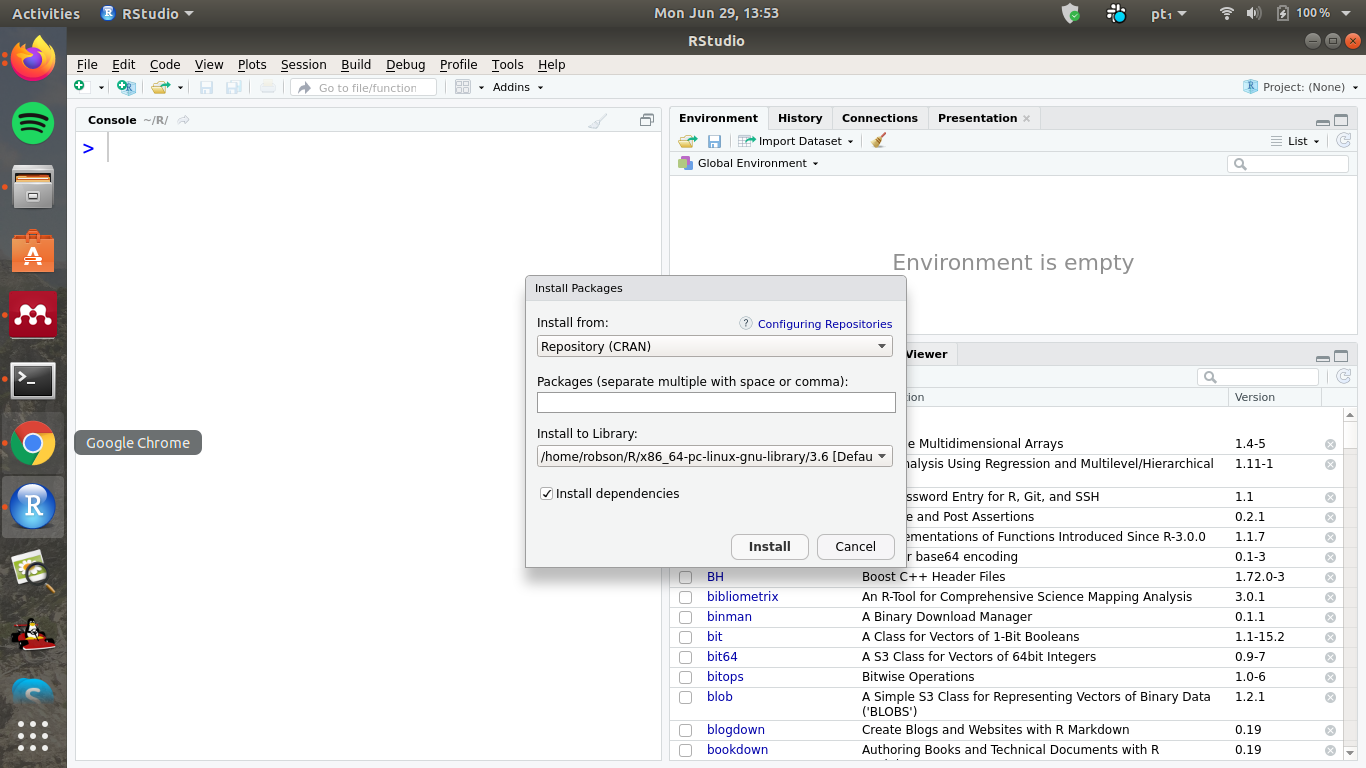
\includegraphics{fig/install_packages_rstudio_visual.png}
\caption{Selecoinar aba de instalação \emph{Packages - Click em install}}
\end{figure}

\begin{enumerate}
\def\labelenumi{\arabic{enumi}.}
\setcounter{enumi}{2}
\tightlist
\item
  No ambiente de busca da interface instalação pesquise
  por \emph{bookdown}, selecione o pacote e clique em \emph{install},
\end{enumerate}

\begin{figure}
\centering
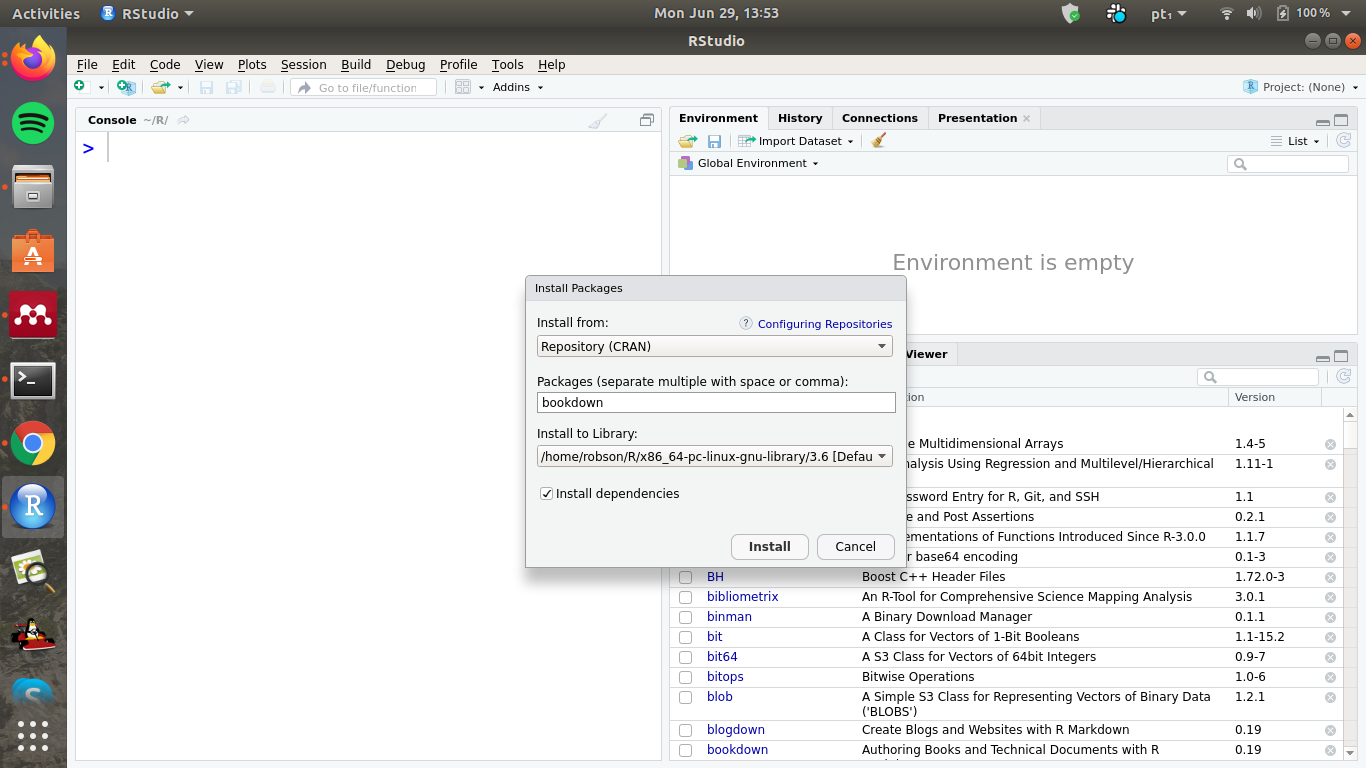
\includegraphics{fig/install_packages_rstudio_visual_bookdown.png}
\caption{\emph{Pesquisar por bookdown e clicar em install}}
\end{figure}

\begin{enumerate}
\def\labelenumi{\arabic{enumi}.}
\setcounter{enumi}{3}
\item
  Finalmente, o código será instalado,
  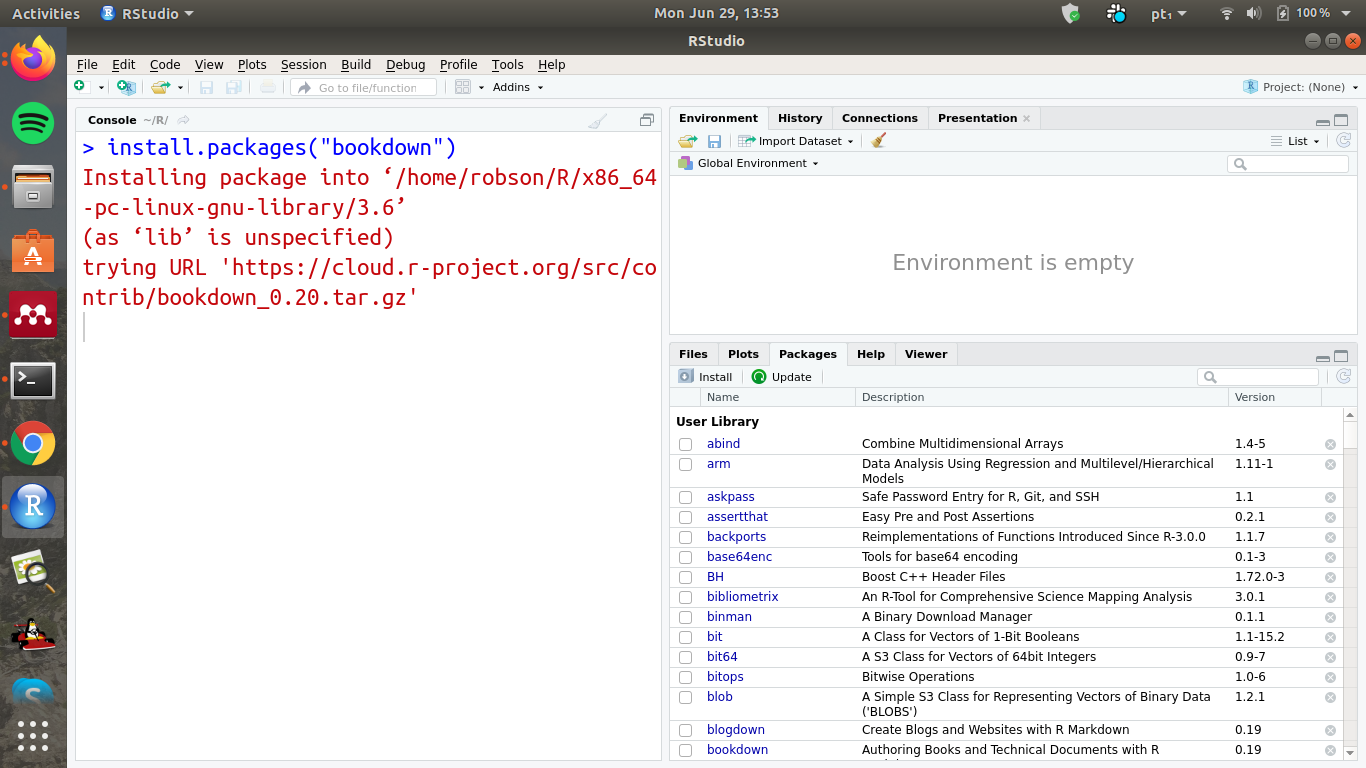
\includegraphics{fig/install_packages_rstudio_visual_bookdown_run.png}
\item
  Ainda é necessário carregá-lo na seção de uso, novamente na aba \emph{Packages} pesquise por \emph{bookdown}
  e selecione o pacote, o que será suficiente para
  carregá-lo,
\end{enumerate}

\begin{figure}
\centering
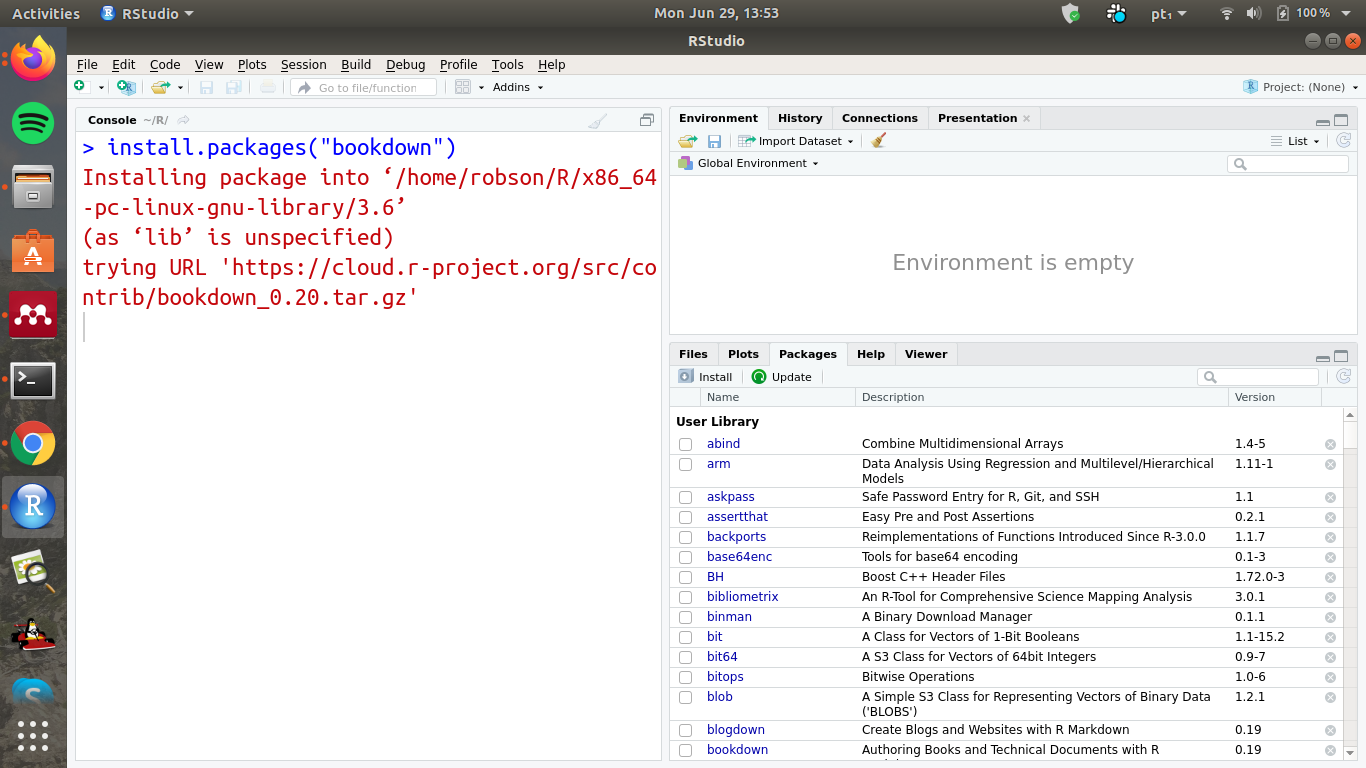
\includegraphics{fig/install_packages_rstudio_visual_bookdown_run.png}
\caption{Carregar a biblioteca bookdown na aba Package}
\end{figure}

\begin{Shaded}
\begin{Highlighting}[]
\KeywordTok{install.packages}\NormalTok{(}\StringTok{"bookdown"}\NormalTok{)}
\CommentTok{# or the development version}
\CommentTok{# devtools::install_github("rstudio/bookdown")}
\KeywordTok{library}\NormalTok{(}\StringTok{"bookdown"}\NormalTok{)}
\end{Highlighting}
\end{Shaded}

Deve-se lembrar que para cada arquivo \emph{.Rmd}
só pode ter um capítulo sendo definido pelo primeiro nível
por \texttt{\#}.

Para compilar este exemplo para PDF, é necessário
o pacote XeLaTeX. É recomendável
instalar o TinyTeX (que inclui o XeLaTeX): \url{https://yihui.org/tinytex/}.

Nos próximos capítulos serão apresentados outros
detalhes sobre instalação e configuração.

\hypertarget{c02}{%
\chapter{Introdução}\label{c02}}

A primeira palavra que devemos pensar
ao encarar um curso de ferramentas de
escrita de textos é \emph{oportunidade}.

Quando pensamos em texto simples e rápidos,
podemos naturalmente usar ferramentas como
WYSIWYG (\emph{What You See Is What You Get})
como \textbf{LibreOffice Writer} ou
\textbf{Microsof Office Word}. Entretanto,
trabalhar com textos longos, como relatórios,
trabalhos de conclusão de curso (TCC),
dissertações ou teses pode exigir
recursos mais avançados como LaTeX.

\hypertarget{criauxe7uxe3o-do-projeto-do-livro}{%
\section{Criação do projeto do livro}\label{criauxe7uxe3o-do-projeto-do-livro}}

Faremos uso mais uma vez de recursos
gráficos da interface do \emph{Rstudio}
para a criação do projeto do livro.
Este material foi prepara utilizando
a estrutura mínima disponibilizada pelo
\emph{template} do pacote \emph{bookdown}.
As etapas a seguir serão o suficiente
para entender a criação e uso desse \emph{template}:

\begin{enumerate}
\def\labelenumi{\arabic{enumi}.}
\tightlist
\item
  Após a instalação e carregamento da biblioteca
  \emph{bookdown}, podemos utilizar o \emph{template},
  primeiro devemos clicar no canto superior direito em \emph{projetos} como:
\end{enumerate}

\begin{figure}
\centering
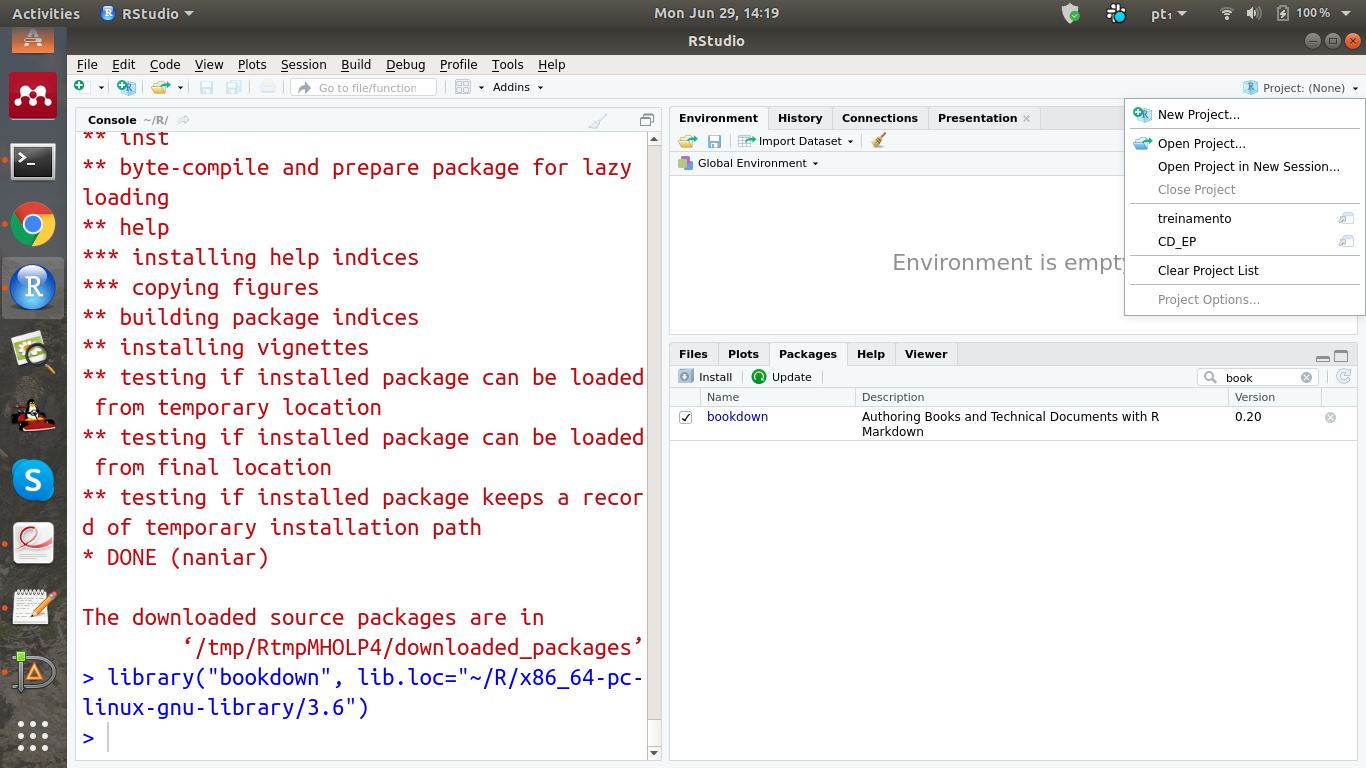
\includegraphics{fig/rstudio_select_new_Project.png}
\caption{Criação de um novo projeto de livro}
\end{figure}

\begin{enumerate}
\def\labelenumi{\arabic{enumi}.}
\setcounter{enumi}{1}
\tightlist
\item
  Em seguida, selecionar \emph{New Directory}:
\end{enumerate}

\begin{figure}
\centering
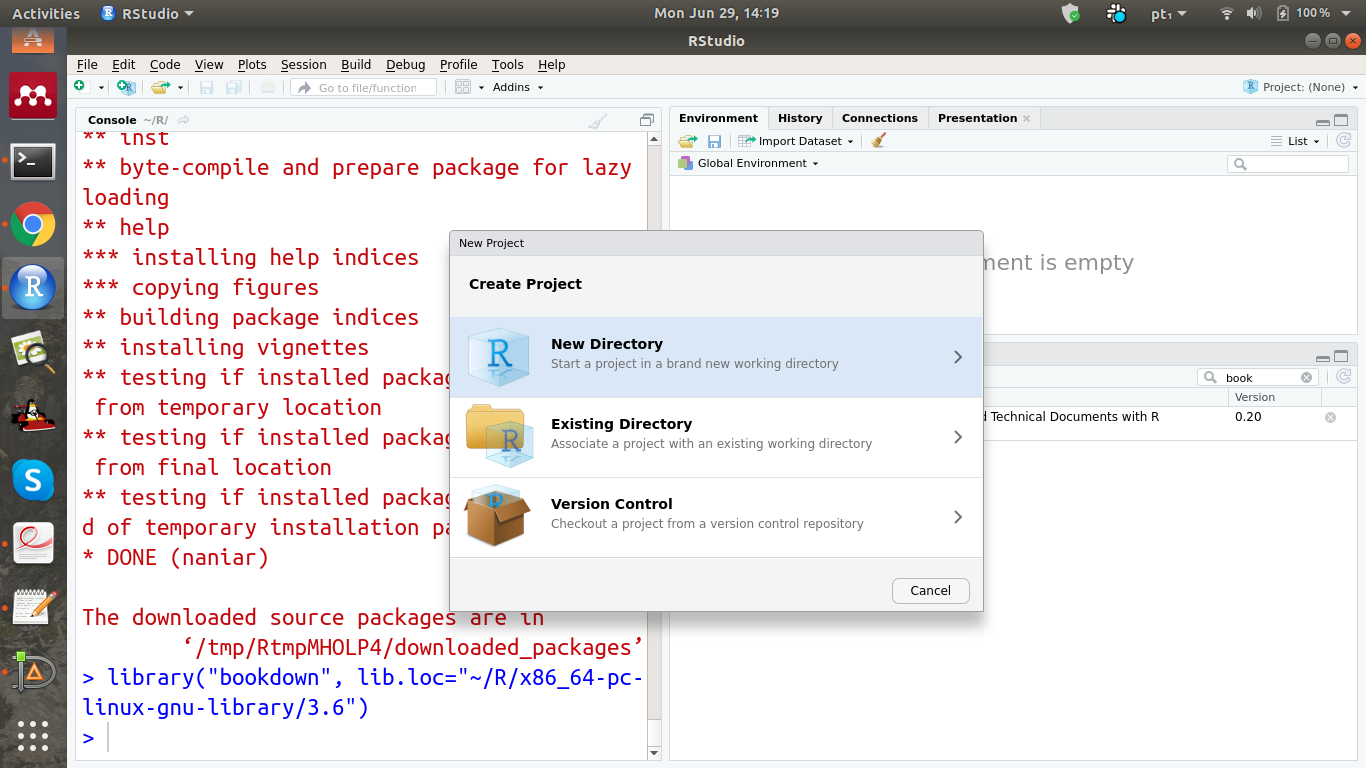
\includegraphics{fig/select_new_directory.png}
\caption{Selecionar a criação de um novo diretório}
\end{figure}

\begin{enumerate}
\def\labelenumi{\arabic{enumi}.}
\setcounter{enumi}{2}
\tightlist
\item
  Selecionar \emph{Book Project with bookdown}
\end{enumerate}

\begin{figure}
\centering
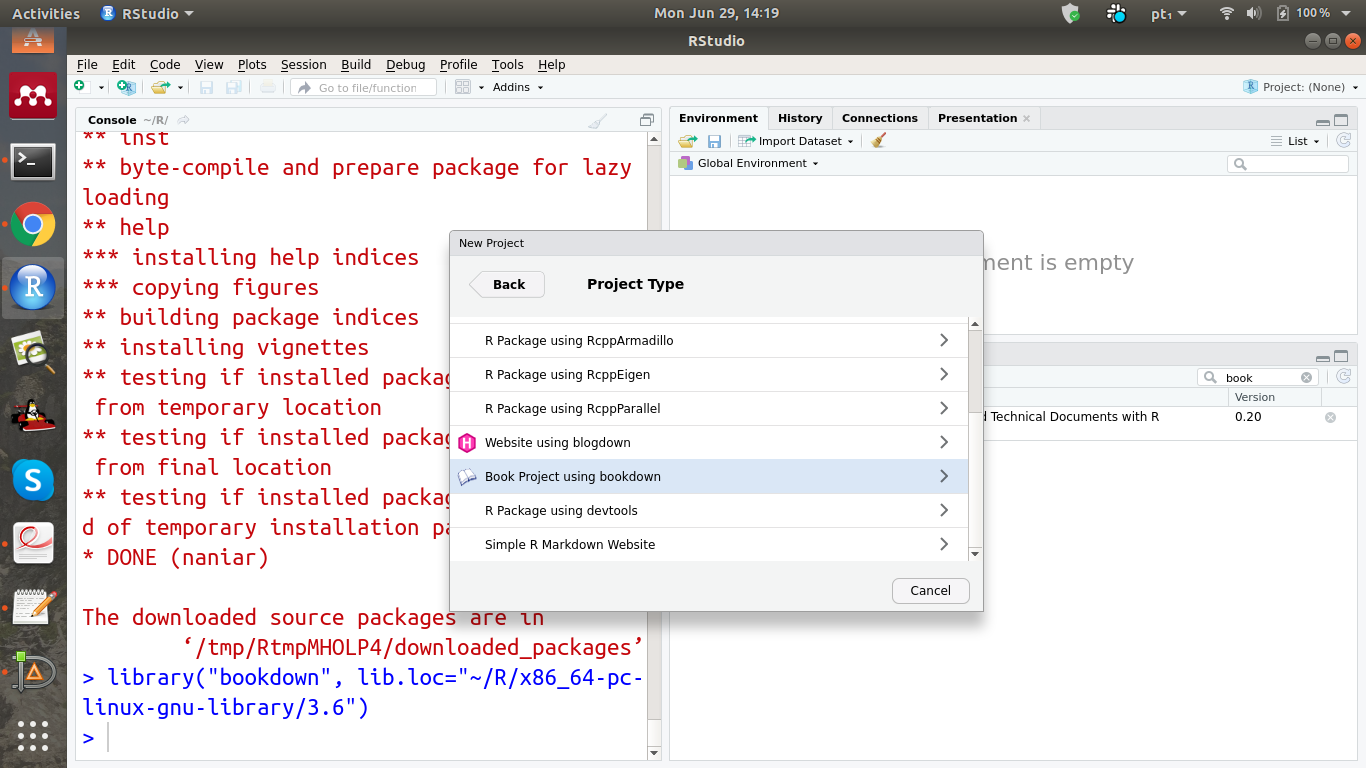
\includegraphics{fig/select_Book_Project_with_bookdown.png}
\caption{Seleção da opção de projeto de livro com pacote bookdown}
\end{figure}

\begin{enumerate}
\def\labelenumi{\arabic{enumi}.}
\setcounter{enumi}{3}
\tightlist
\item
  Em seguida o template com a versão mínima será
  disponibilizado por meio de uma pasta com o nome escolhido na etapa anterior.
\end{enumerate}

\begin{figure}
\centering
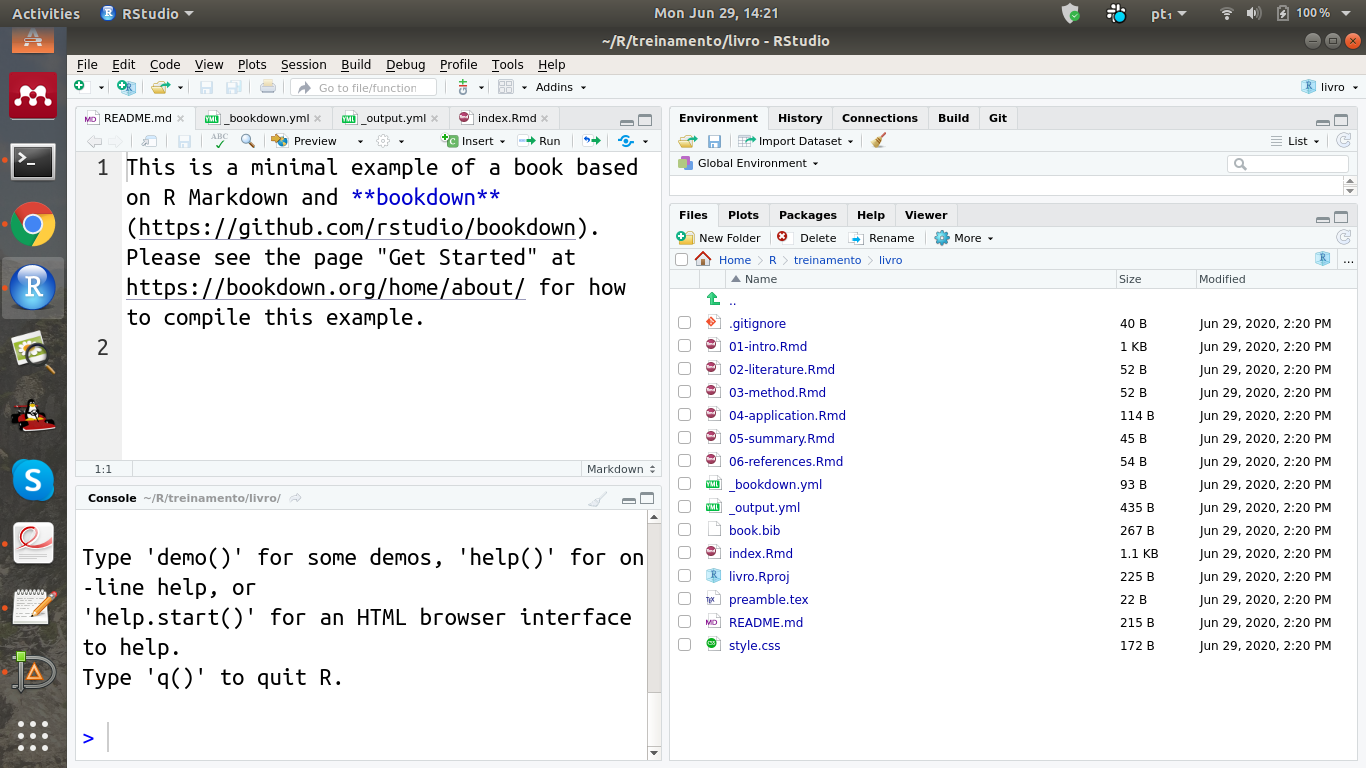
\includegraphics{fig/outra.png}
\caption{Seleção da opção de projeto de livro com pacote bookdown}
\end{figure}

Na lista apresentada acima são identificados
arquivos com as seguintes extensões:

\begin{itemize}
\tightlist
\item
  \textbf{.Rmd}
\item
  \textbf{.bib}
\item
  \textbf{.yml}
\item
  \textbf{.tex}
\item
  \textbf{.css}
\end{itemize}

Aqueles arquivos cuja a extensão é \emph{.Rmd}
são utilizados para a escrita dos
conteúdos do livro em R Markdown. Entretanto,
entre eles
há um especial, \emph{index.Rmd}, que constrói
a página principal, por meio de
comandos \textbf{yml}. Algumas configurações
são reservadas em dois arquivos com extensão
\textbf{.yml}. Sendo o arquivo \_bookdown.yml para
configurações gerais que serão úteis para quaisquer
tipo de documento de saída, por exemplo, a definição
se o título de cada capítulo será chamado de
\textbf{Chapter } ou \textbf{Capítulo }, especialmente
para este treinamento fizemos esta alteração. Enquanto
que para o arquivo *\_output.yml* são apresentadas
configurações especiais para cada tipo de saída,
como \emph{bookdown::gitbook}, \emph{bookdown::pdf\_book:} ou
\emph{bookdown::epub\_book:}. Especialmente para o
caso do \emph{gitbook} é necessário a existência do arquivo
\emph{style.css} para algumas configurações. Já o arquivo
\emph{book.bib} é uma estrutura especial do pacote \emph{bibtex}
do LaTeX e contem as informações de artigos que serão citados.

\hypertarget{c03}{%
\chapter{Visualização e Ciência de dados}\label{c03}}

O capítulo \ref{c02} apresenta a tabela como uma forma poderosa para estruturar e visualizar informações. No entanto, quando trabalhamos com enormes tabelas com uma imensa quantidade de linhas e colunas se torna difícil interpretar suas informações, não importa o quão organizadas elas estejam. Às vezes, é muito mais fácil interpretar essas informações através dos gráficos, conteúdo que será explorado no decorrer deste capítulo.

A construção e visualização gráfica é de extrema importância na área de ciência de dados, pois é a partir de um bom gráfico que podemos extrair ideias, hipóteses e um melhor entendimento a respeito de um tema ou uma pergunta. A importância desse tipo de análise pode ser expressa por um ditado popular bastante conhecido: ``Uma imagem vale mais que mil palavras''.

\hypertarget{objeto-de-estudo-do-capuxedtulo}{%
\section{Objeto de Estudo do capítulo}\label{objeto-de-estudo-do-capuxedtulo}}

Para compreender a importância da análise gráfica e como utiliza-la corretamente, iremos analisar o perfil dos estudantes de Salvador que realizaram a prova do Exame Nacional do Ensino Médio (ENEM) no período de 2015 até 2019.

Porém, antes de qualquer coisa: O que é um \textbf{Perfil}? Esse termo é muito usado na estatística para \textbf{descrever determinado processo ou objeto de estudo, buscando entender características e padrões que o representa}. Para este caso em específico, vamos estudar os estudantes da cidade de Salvador utilizando os microdados do ENEM, publicados pelo Instituto Nacional de Estudos e Pesquisas Educacionais Anísio Teixeira (INEP), disponível ao público através deste \href{http://inep.gov.br/microdados}{link de acesso}.

Como o termo \textbf{perfil} pode ser bem vasto e diversas características podem ser extraídas, é necessário concentrar essa análise em perguntas mais específicas para nortear o estudo. No decorrer deste capítulo, será explorado graficamente as seguintes questões:

\begin{itemize}
\item
  A quantidade de estudantes que realizam o ENEM aumentou de 2015 para 2019 na capital bahiana?
\item
  Como é a distribuição de estudantes em Salvador por cor/raça? Conseguimos identificar algum padrão para esses valores?
\item
  Na era da informação, como está o acesso dos estudantes a internet em suas residências?
\item
  O acesso a computadores pessoais é algo comum para os estudantes de Salvador?
\item
  O tipo de escola (pública ou privada) pode influenciar nas notas dos estudantes neste exame?
\end{itemize}

A compreensão desses dados é de suma importância para compreender melhor o perfil dos estudantes de Salvador que possuem o ENEM como uma oportunidade de acesso, as vezes única, ao ensino superior no Brasil.

\hypertarget{gruxe1fico-de-barra}{%
\section{Gráfico de barra}\label{gruxe1fico-de-barra}}

O \textbf{Gráfico de barras} é uma forma bastante comum e versátil de visualização na área de ciência de dados. Ele pode ser utilizado tanto com variáveis categóricas quanto numéricas para expressar grandezas. A Figura abaixo apresenta uma de suas utilizações: demonstrar grandezas numéricas.

\begin{figure}

{\centering 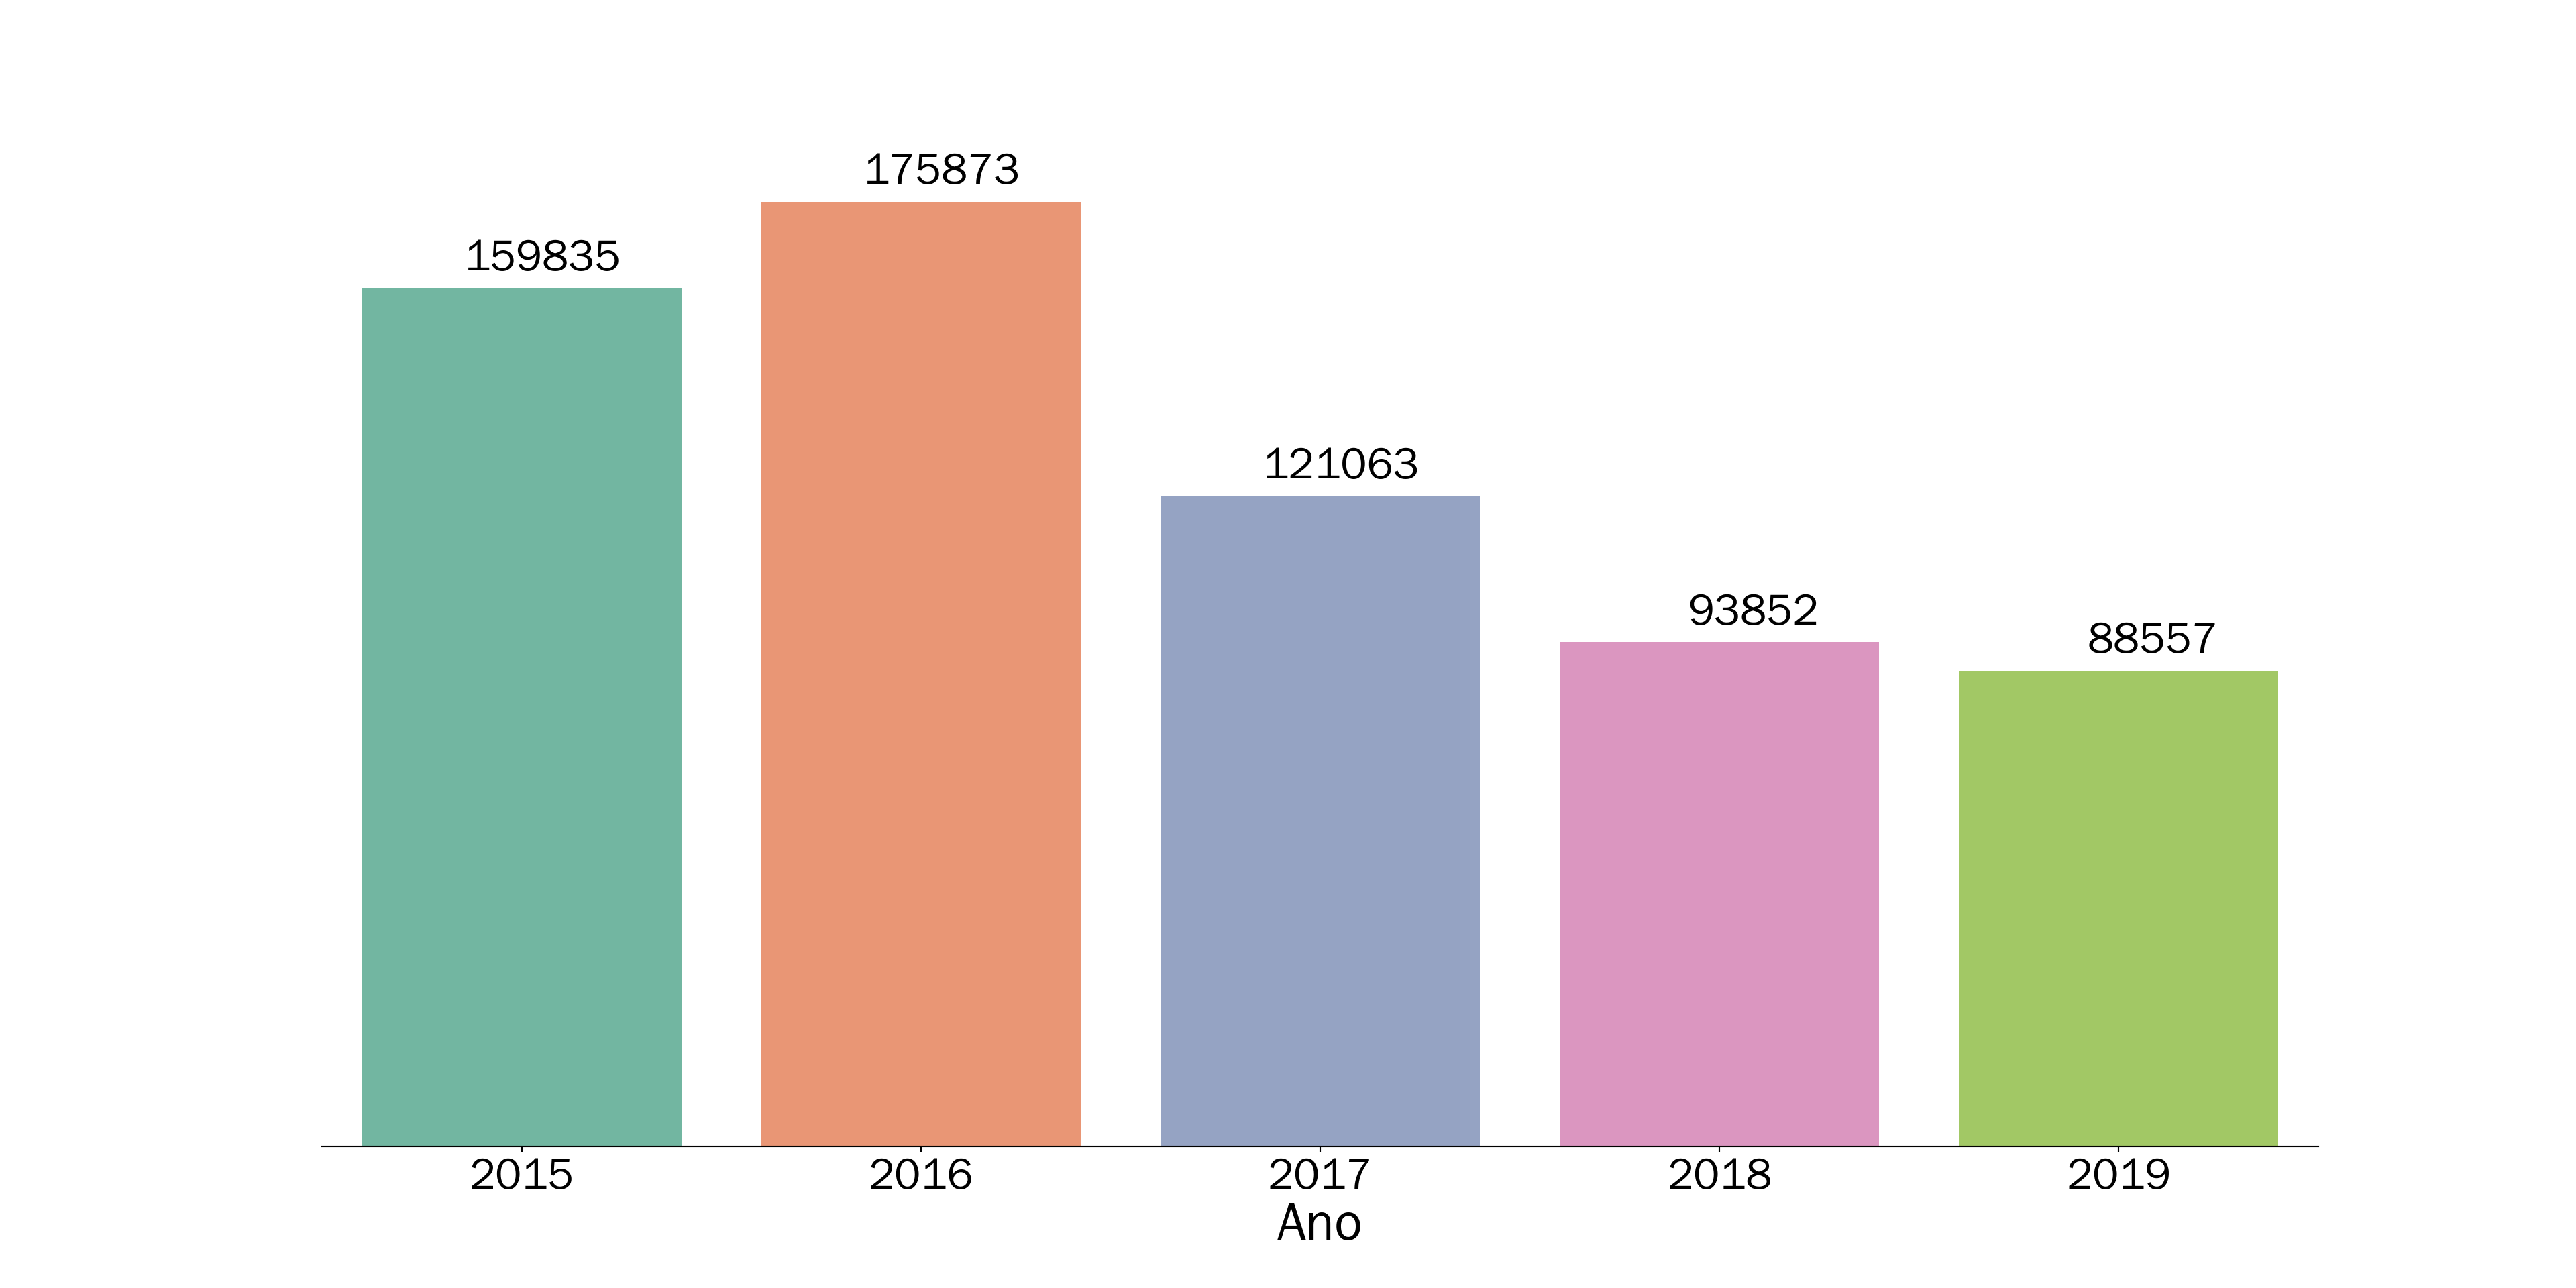
\includegraphics[width=1\linewidth]{livro_files/figure-latex/f31-1} 

}

\caption{Quantidade de estudantes que realizaram o ENEM na capital bahiana}\label{fig:f31}
\end{figure}

Na Figura \ref{fig:f31} é apresentado a quantidade de estudantes que realizaram o ENEM de 2015 até 2019 na capital bahiana. É possível notar uma queda drástica na participação de estudantes entre os períodos de 2016 até 2019. Apesar de simples e direto, a análise desse mesmo resultado através de uma tabela pode se mostrar confusa:

\begin{longtable}[]{@{}cc@{}}
\toprule
Ano & Número de estudantes em Salvador\tabularnewline
\midrule
\endhead
2015 & 159835\tabularnewline
2016 & 175873\tabularnewline
2017 & 121063\tabularnewline
2018 & 93852\tabularnewline
2019 & 88557\tabularnewline
\bottomrule
\end{longtable}

Note que ao visualizar a Tabela, nenhuma informação visual é passada para destacar os anos com mais ou menos participantes. Além disso, ela contém as mesmas informações demonstradas na Figura \ref{fig:f31}, porém com uma diferença: através da visualização gráfica fica muito mais claro a queda de inscrições no ENEM de 2016 até 2019.

O gráfico de barras apresenta uma característica muito importante relacionado ao tamanho das barras: elas crescem proporcionalmente de acordo as grandezas que elas se referem, ou seja, quanto maior o valor maior será sua barra. Comumente essas barras apresentam a mesma largura neste tipo de gráfico.

É através da Figura \ref{fig:f31} que podemos responder a primeira pergunta:\textbf{A quantidade de estudantes que realizam o ENEM aumentou de 2015 para 2019 na capital bahiana?} E a resposta é não. Apesar do número de estudantes crescer de 2015 para 2016, ocorre uma queda drástica até 2019, chegando a diminuir pela metade o número de inscrições em Salvador.

Essa resposta pode te levar a um questionamento mais profundo: O que realmente motivou essa queda?. Infelizmente encontrar a resposta para este questionamento não é trivial, requer pesquisas mais específicas a cerca do tema, o que foge do escopo deste capítulo. Todavia, é interessante refletir como a partir de um gráfico simples, podemos alcançar perguntas ainda mais complexas.

Agora que respondemos a primeira questão, podemos perceber que a pergunta ``\textbf{Como é a distribuição de estudantes em Salvador por cor/raça? Conseguimos identificar algum padrão para esses valores?}'' está bastante relacionada ao seu resultado.
Inicialmente para entender essa relação, precisamos entender o que seria essa distribuição de raças no questionário no ENEM. Trata-se de uma pergunta que busca entender como o estudante se classifica em relação a sua cor. Essa pergunta possui 7 respostas possíveis:

\begin{itemize}
\item
  Não declarado
\item
  Pardo
\item
  Preta
\item
  Branco
\item
  Amarelo
\item
  Indígena
\item
  Opção de não apresentar tal informação
\end{itemize}

Como foi explicado no Capítulo \ref{c02}, esse questionamento pode ser definido como uma variável categórica. Ele está bastante relacionada com a primeira questão, pois a quantidade de total de estudantes pode alterar essa distribuição, aumentando ou diminuindo a depender das categorias. Como tivemos uma diferença tão grande entre o número de inscritos em 2016 e 2019 demonstrado na Figura \ref{fig:f31}, uma análise mais aprofundada nesses dois anos podem trazer resultados interessantes para responder nosso segundo questionamento:

\begin{figure}

{\centering 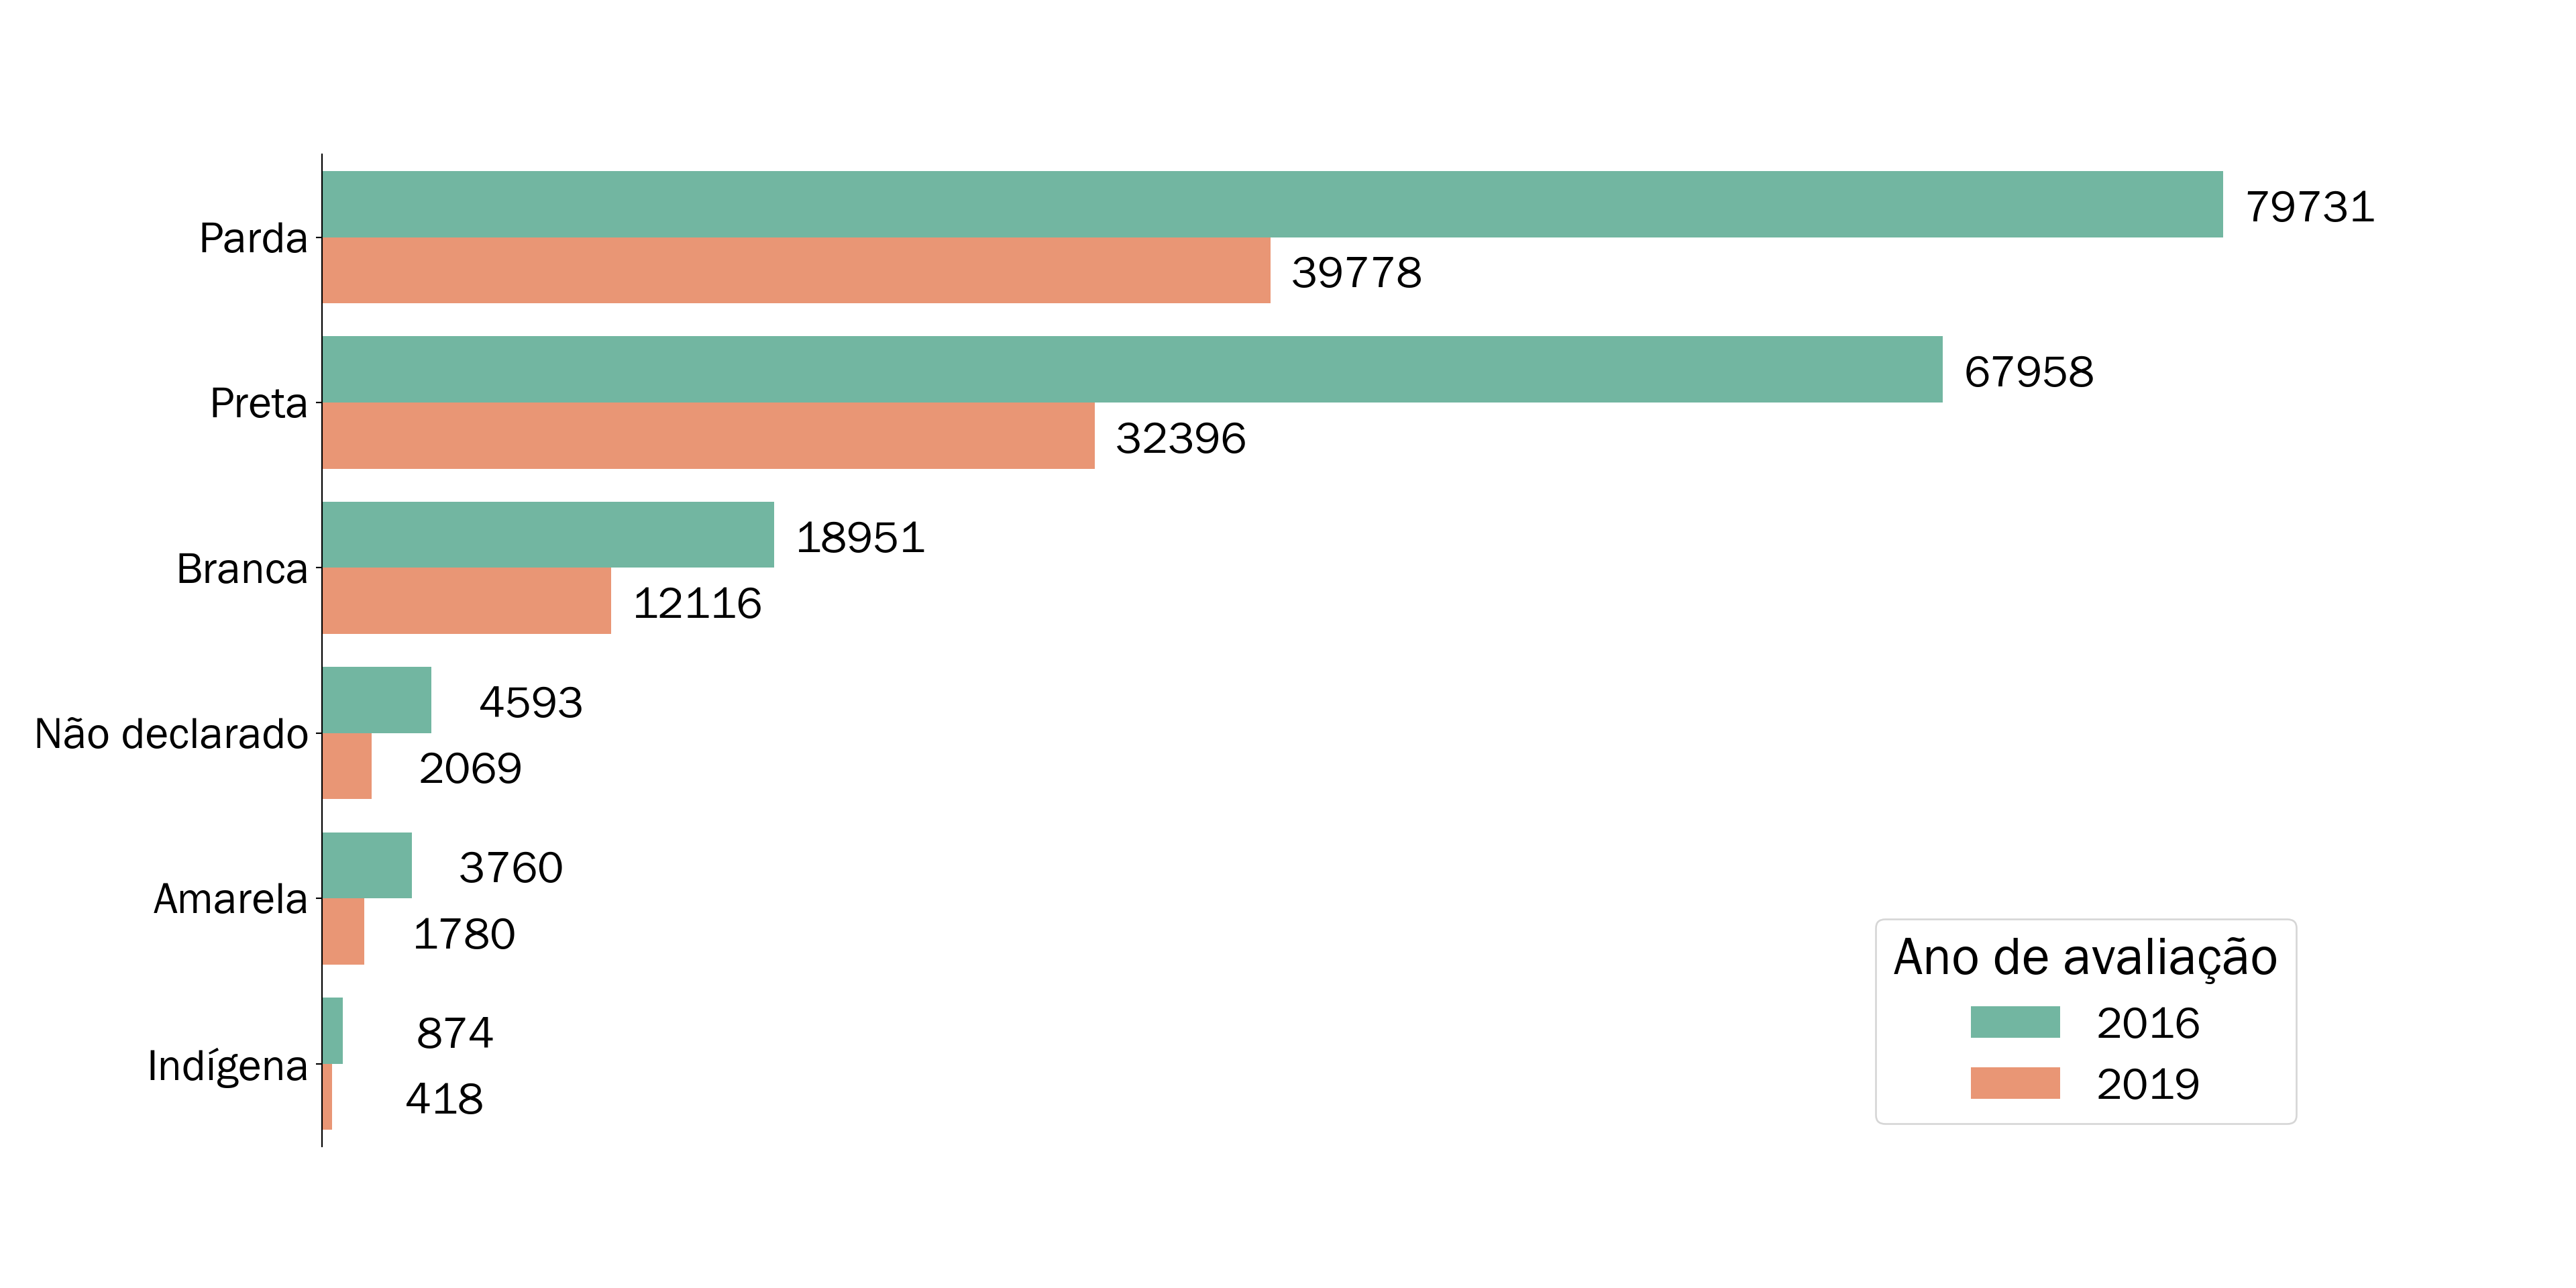
\includegraphics[width=1\linewidth]{livro_files/figure-latex/f32-1} 

}

\caption{Distinção de estudantes por cor/raça da cidade de Salvador para os anos de 2016 e 2019}\label{fig:f32}
\end{figure}

Através da Figura \ref{fig:f32}, é apresentado os valores absolutos da quantidade de estudantes que realizaram o ENEM em cada ano identificados pela sua raça. Note que a grande queda encontrada na Figura \ref{fig:f31} se reflete neste gráfico também: Em comparação a 2016, todas as categorias apresentaram valores menores. Por exemplo, a quantidade pessoas pardas que realizaram o ENEM caiu quase pela metade, assim como pessoas auto-declaradas como preta. Além disso, podemos notar uma baixíssima quantidade de pessoas indígenas/amarela que realizam este exame e que em sua grande maioria, os estudantes da capital bahiana se declaram como pardos e negros. Essa situação já era esperada e reflete uma realidade já conhecida: Segundo o Instituto Brasileiro de Estatística e Geografia (IBGE), em uma \href{https://www.acordacidade.com.br/noticias/203087/ibge-ba-salvador-a-capital-mais-negra-do-brasil-e-com-a-maior-desigualdade-salarial-entre-brancos-e-pretos.html?mobile=true}{pesquisa realizada em 2017}, Salvador é considerada a capital mais preta do brasil, onde 8 em cada 10 moradores se autodeclaravam de cor preta ou parda.

Note que a Figura \ref{fig:f32} demonstra também a principal função do gráfico de barras: dimensionar variáveis categóricas de acordo a frequência de suas categorias. \textbf{Frequência} para uma variável categórica pode ser definido com a quantidade de vezes que ela é representada, podendo ser dividida em dois tipos: absoluta e relativa.

A frequência absoluta se trata da representação da quantidade de vezes que cada categoria ocorre. Este tipo de frequência é trabalhada na Figura \ref{fig:f32}, onde apresentamos a quantidade de estudantes por cor/raça que realizaram o ENEM nos anos de 2016 e 2019. Ainda na Figura \ref{fig:f32}, conseguimos notar que para todas as categorias apresentaram uma queda na quantidade de estudantes que realizaram em 2016 para 2019, mas e se quisermos comparar este valores ainda utilizando um gráfico de barras, seria possível?

Uma boa forma para comparar essas frequências absolutas distintas seria através do segundo tipo de frequência apresentada anteriormente: a frequência relativa. A frequência relativa é definida como uma proporção entre o valor que você quer estimar e o valor máximo esperado. Podemos formular este conceito da seguinte forma:
\[Frequência\ Relativa (\%) = 100*{Valor\ para\ comparar \choose Valor\ máximo}\]
Note que não foi mencionado o valor \(100\) presente na fórmula. Ele é apresentado para tornar o resultado da frequência relativa em porcentagem. Para compreender melhor este conceito apresentado, vamos continuar respondendo a segunda questão utilizando agora este novo aprendizado:

\begin{figure}

{\centering 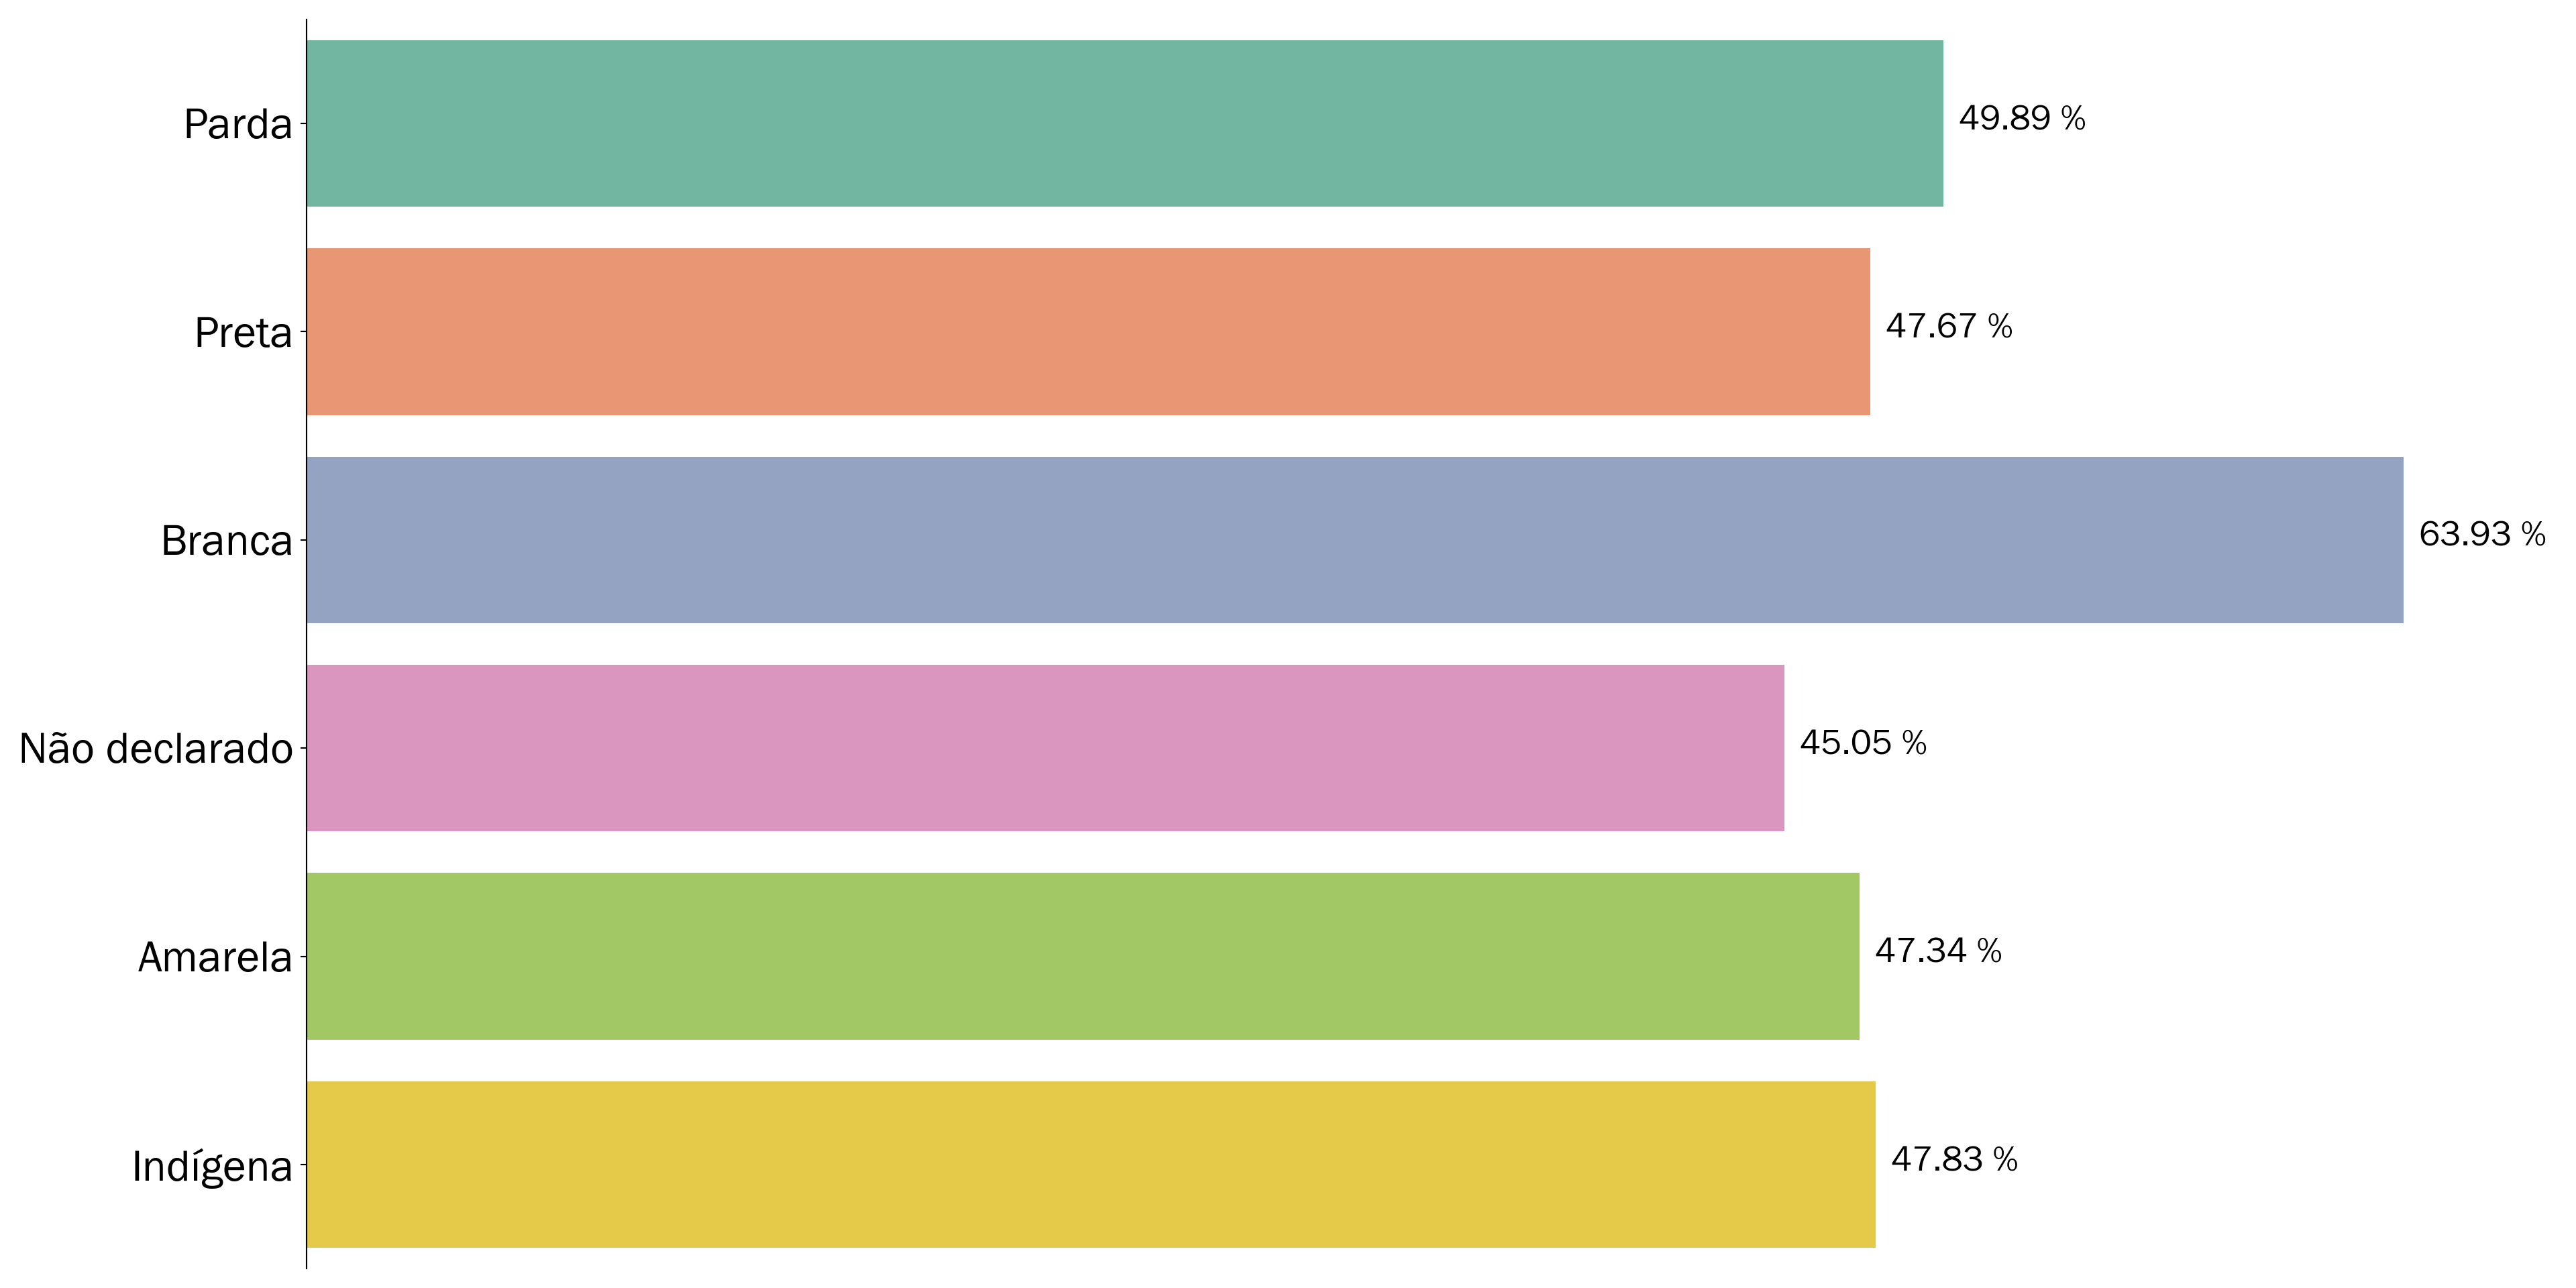
\includegraphics[width=1\linewidth]{livro_files/figure-latex/f33-1} 

}

\caption{Comparação entre os estudantes de Salvador por cor/raça para 2016 e 2019}\label{fig:f33}
\end{figure}

A Figura \ref{fig:f33} pode ser vista como uma extensão da Figura \ref{fig:f32}, utilizando a frequência relativa para apresentar uma informação implícita: a proporção dos estudantes que fizeram o ENEM em 2019 em comparação a quantidade que realizaram o exame em 2016. Transcrevendo a fórmula da frequência relativa apresentada anteriormente, temos:
\[Frequência\ Relativa (\%) = 100*{Quantidade\ de\ estudantes\ \ realizaram\ o\ ENEM\ em\ 2019\choose Quantidade\ de\ estudantes\ \ realizaram\ o\ ENEM\ em\ 2016}\]
Como nos é apresentado uma proporção, podemos ler o gráfico de barras apresentado na Figura \ref{fig:f33} como sendo \textbf{a quantidade de estudantes que fizeram a prova em 2019 em relação a quantidade que realizaram a prova em 2016}. Podemos identificar, por exemplo, que com exceção dos estudantes auto-declarados de cor branca todas as outras cores apresentaram uma proporção de aproximadamente 50\%, ou seja, o número de estudantes pardos, pretos, amarelos, indígenas e não declarados caíram pela metade em comparação ao ano de 2016. Esta informação intensifica ainda mais o resultado apresentado na Figura \ref{fig:f31}.

Através da análise do gráfico de barras conseguimos avaliar dois questionamentos de uma só vez! Porém para analisar como esses resultados ocorreram de 2016 até 2019 ao invés de dois anos separados, qual seria o melhor tipo de gráfico? Iremos explora-lo na próxima seção deste capítulo.

\hypertarget{suxe9ries-temporais}{%
\section{Séries temporais}\label{suxe9ries-temporais}}

\hypertarget{gruxe1fico-de-pizza}{%
\section{Gráfico de pizza}\label{gruxe1fico-de-pizza}}

\hypertarget{gruxe1ficos-de-dispersuxe3o}{%
\section{Gráficos de Dispersão}\label{gruxe1ficos-de-dispersuxe3o}}

\hypertarget{histograma}{%
\section{Histograma}\label{histograma}}

\hypertarget{aprimorando-suas-visualizauxe7uxf5es}{%
\section{Aprimorando suas visualizações}\label{aprimorando-suas-visualizauxe7uxf5es}}

\hypertarget{indo-aluxe9m}{%
\section{Indo Além \ldots{}}\label{indo-aluxe9m}}

\hypertarget{literatura-e-bibtex}{%
\chapter{Literatura e bibtex}\label{literatura-e-bibtex}}

O foco deste capítulo está numa das
principais potencialidades do LaTeX
utilizas pelo R Markdown a capacidade
de citar os documentos adequadamente
organizados num arquivo \emph{.bib},
especialmente neste exemplo aproveitamos
o arquivo gerado pela estrutura mínima
\emph{bookdown}.

Para esta etapa aproveitaremos como exemplo
os artigos do projeto organizados na
plataforma Mendeley, seguindo os
seguintes passos:

\begin{enumerate}
\def\labelenumi{\arabic{enumi}.}
\tightlist
\item
  Abrir Medeley Desktop;
\item
  Abrir pasta do grupo nomeada por CDnaEP;
\item
  Selecionar os artigos que pretende citar no seu documento;
\item
  Clicar com o botão direito do mouse, selecionar \emph{Copy as} e em seguida \emph{BibTex entry}.
\item
  Abrir o arquivo \emph{book.bib} e colar os metadados
  dos artigos na última linha do arquivo depois da
  última chave \textbf{\}}.
\item
  Em seguida, salve e feche o arquivo \emph{book.bib}.
\end{enumerate}

As figuras a seguir estão de acordo com a sequência acima apresentada:

\begin{figure}
\centering
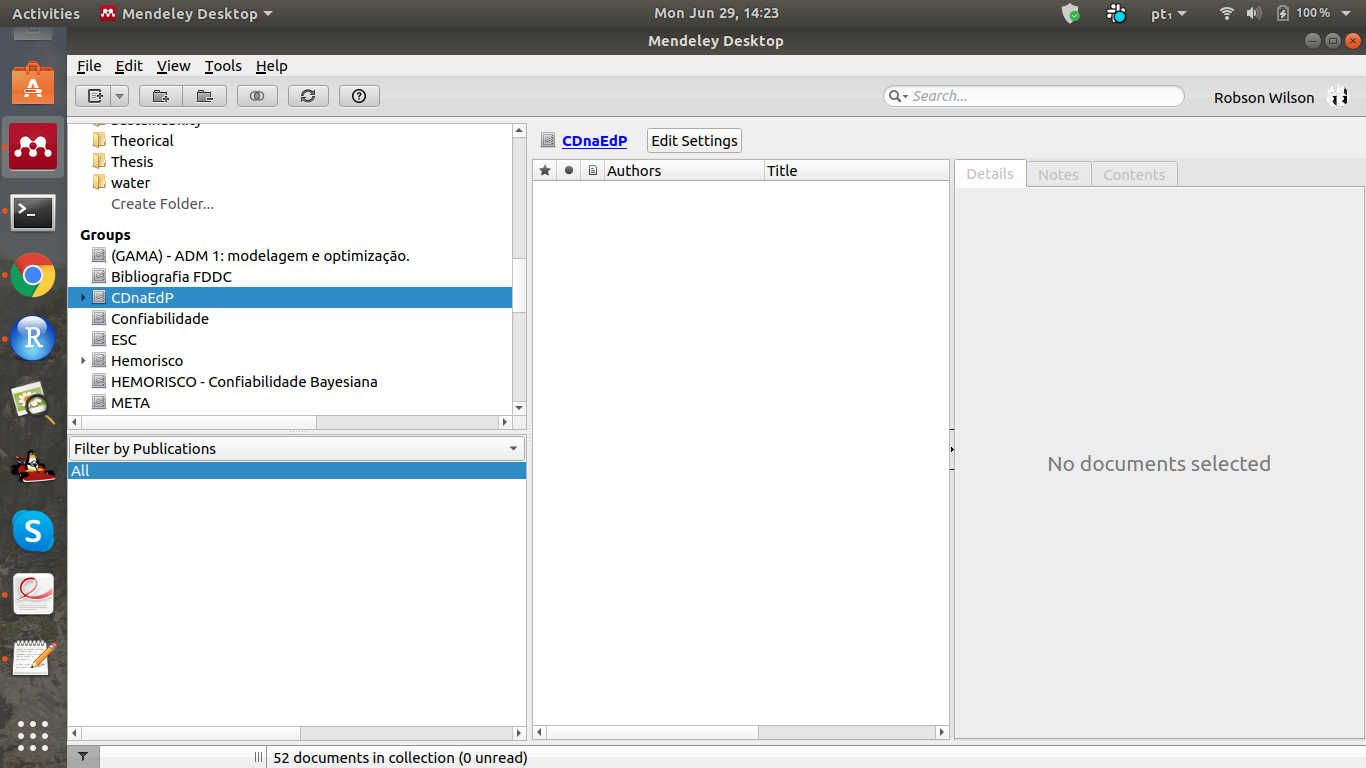
\includegraphics{fig/open_mendeley.png}
\caption{Abrir Medeley Desktop e selecionar pasta CDna EP}
\end{figure}

\begin{figure}
\centering
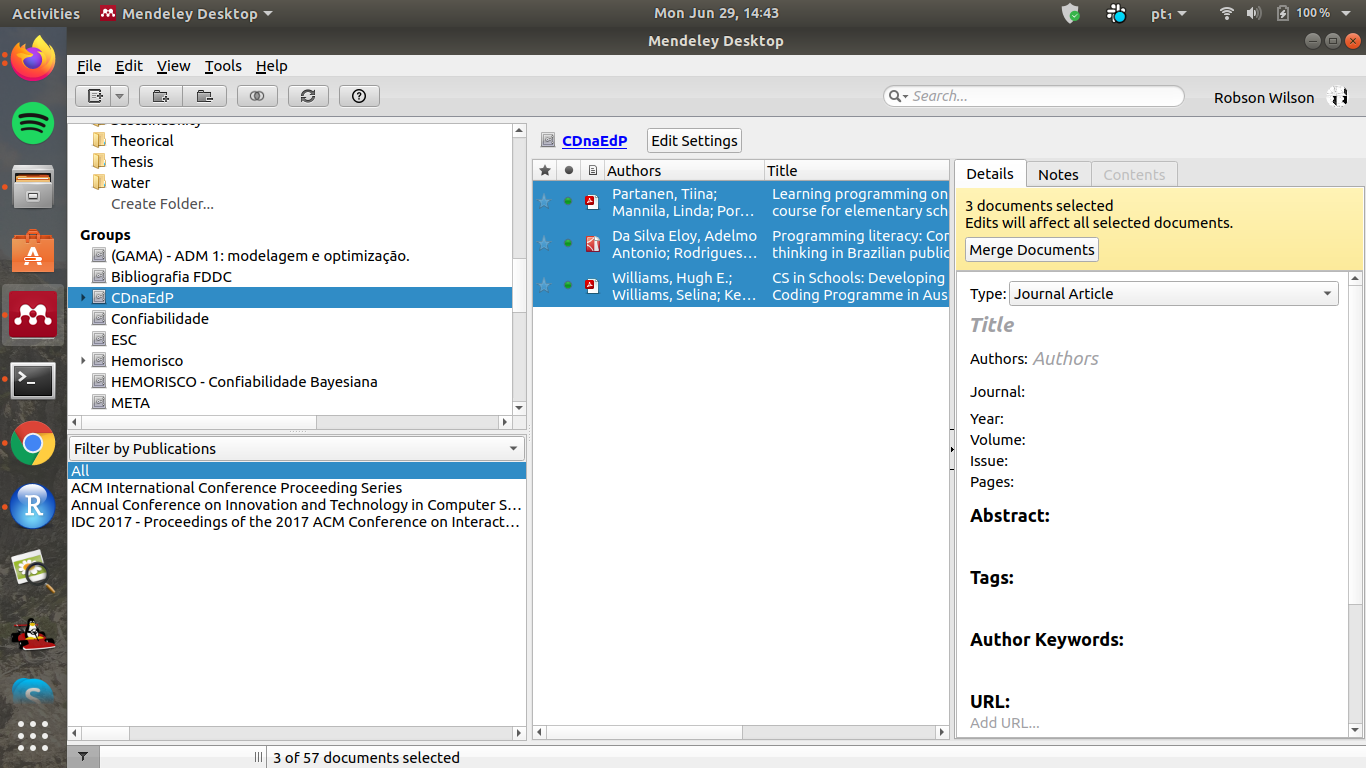
\includegraphics{fig/mendeley_select_CDnaEP_paper_list.png}
\caption{Selecionar artigos para citação}
\end{figure}

\begin{figure}
\centering
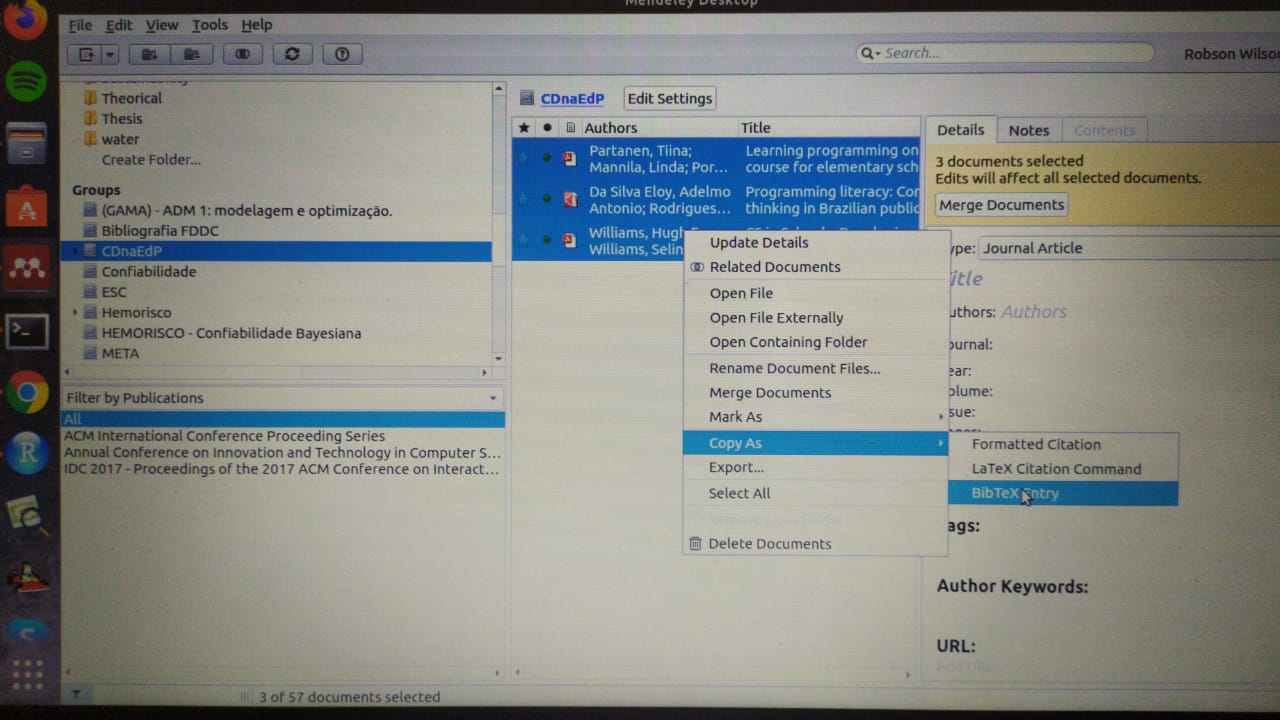
\includegraphics{fig/mendeley_copy_bibtex_entry.jpeg}
\caption{Copiar metadados no formato de entrada do bibtex}
\end{figure}

Uma informação importante para quem ainda não
é familiarizado com LaTeX é o fato
da primeira informação dos metados
de um artigo dentro do arquivo \emph{.bib}
ser a \emph{label}, a informação que será
usada para citações ao longo do documento.

\begin{figure}
\centering
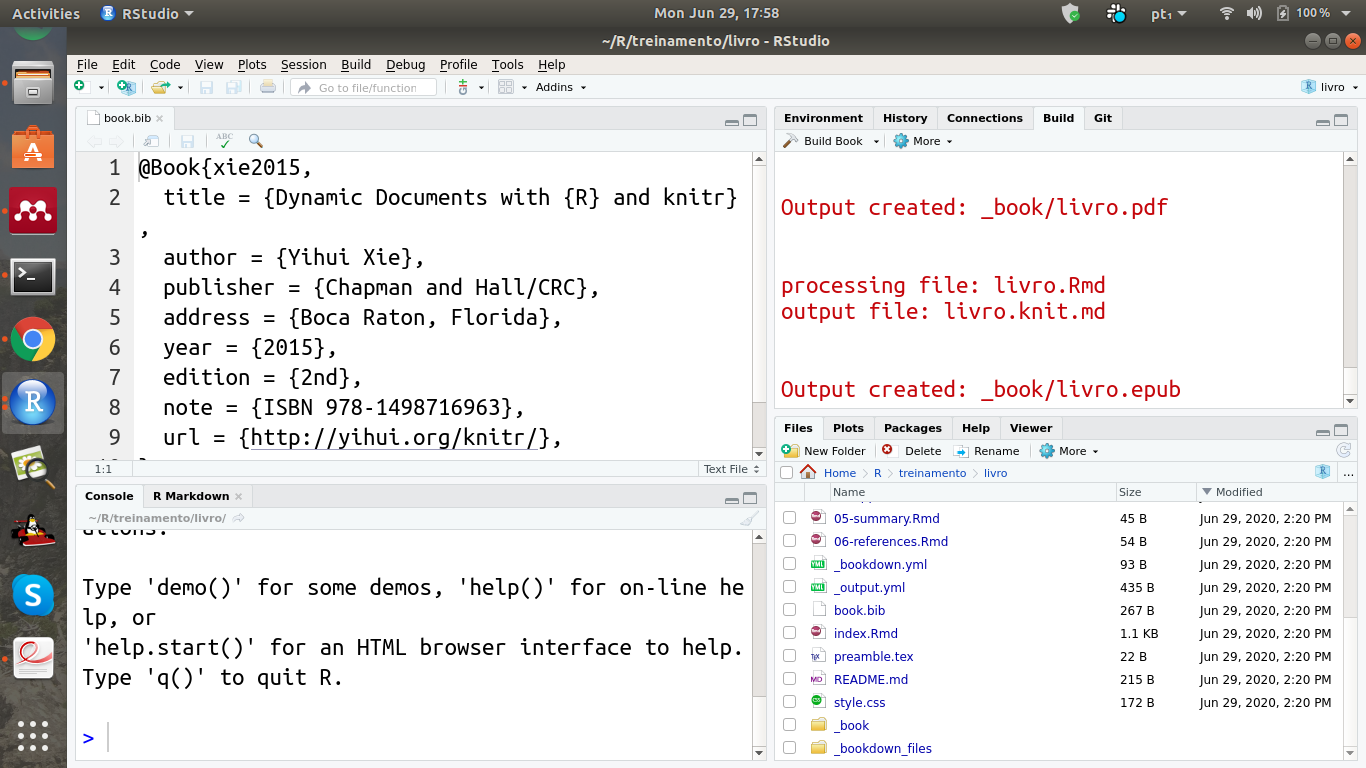
\includegraphics{fig/rstudio_open_bookbib_first.png}
\caption{Identificação da \emph{label} do livro do (\citep{xie2015})}
\end{figure}

\begin{figure}
\centering
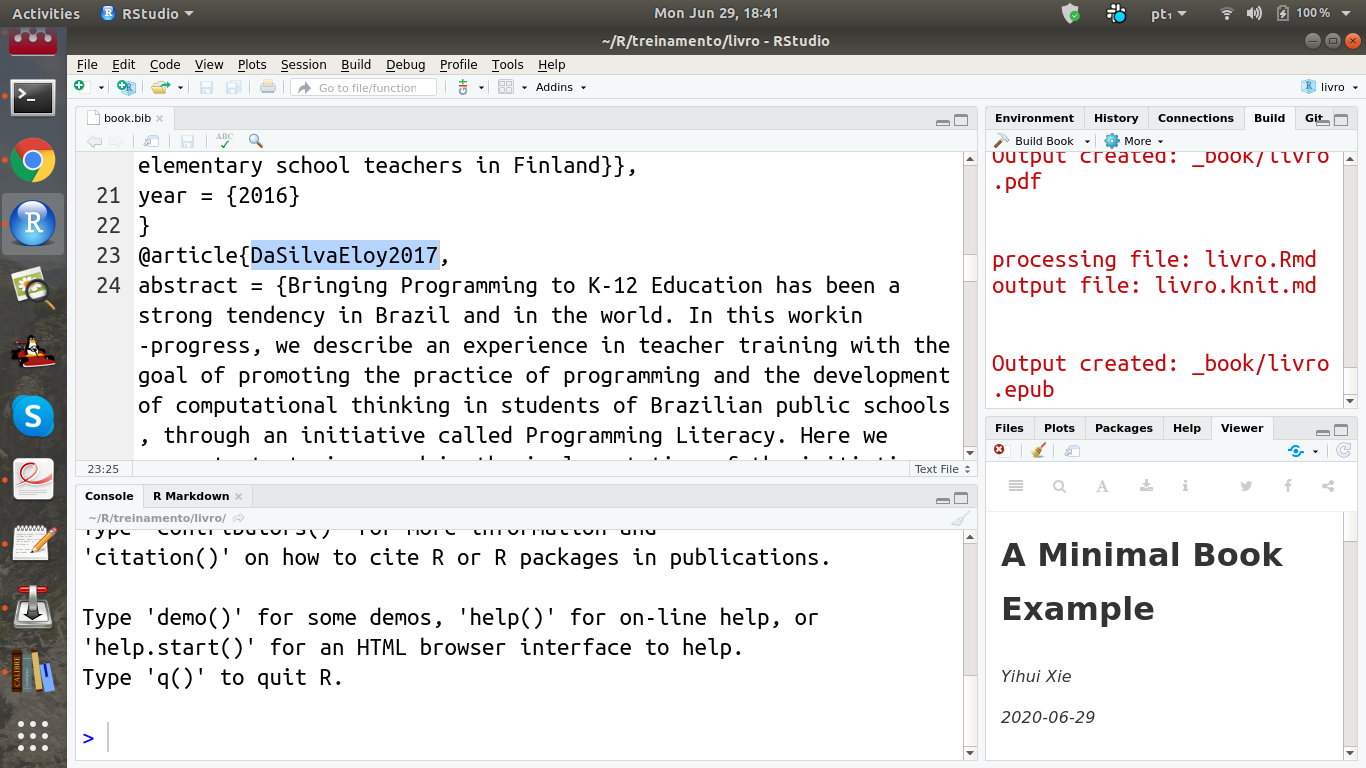
\includegraphics{fig/rstudio_open_bookbib_second.png}
\caption{Identificação da \emph{label} de cada artigo (\citep{DaSilvaEloy2017})}
\end{figure}

\begin{figure}
\centering
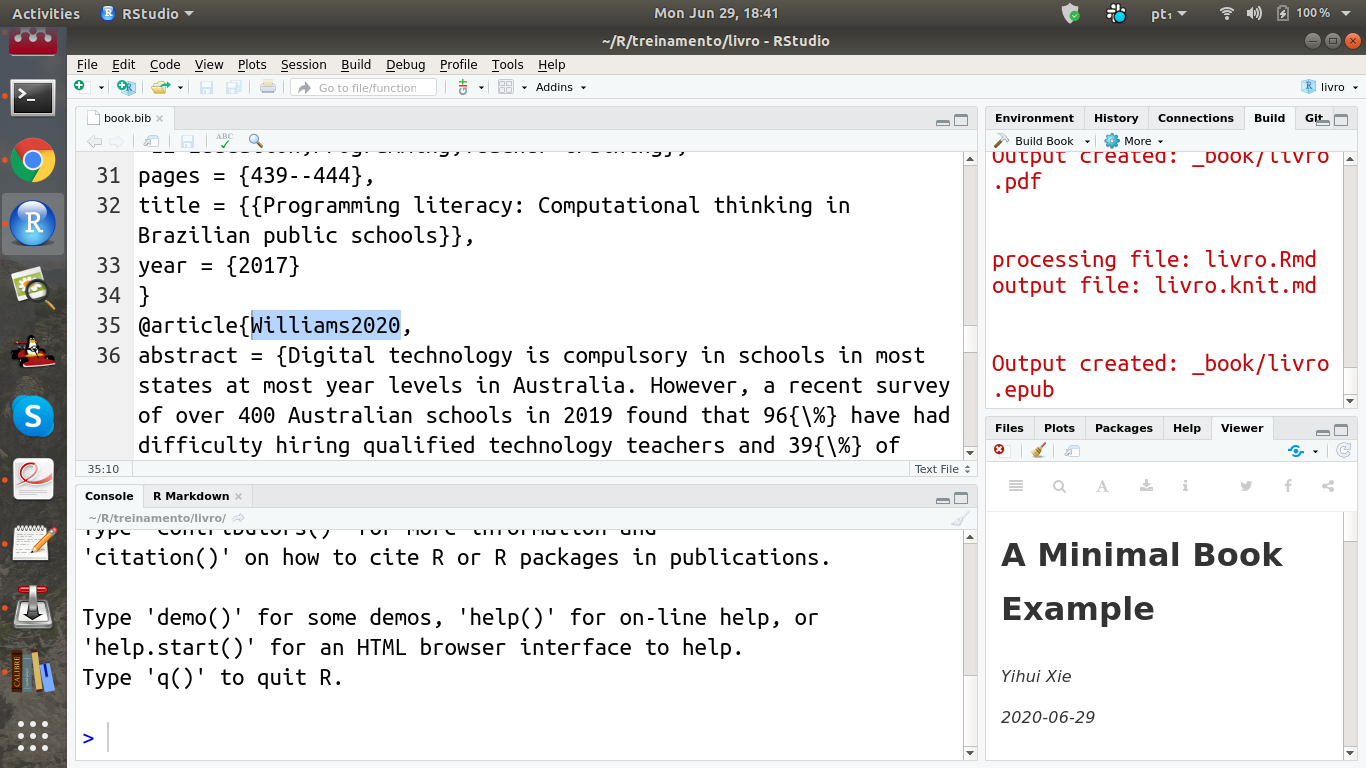
\includegraphics{fig/rstudio_open_bookbib_third.png}
\caption{Identificação da \emph{label} de cada artigo (\citep{Williams2020})}
\end{figure}

Nas subseções a seguir mostramos como citar alguns desses trabalhos.

\hypertarget{exemplo-de-citauxe7uxe3o-simples}{%
\section{Exemplo de citação simples}\label{exemplo-de-citauxe7uxe3o-simples}}

Vamos considerar a citação do artigo \citep{Partanen2016}.

\hypertarget{citauxe7uxf5es-de-dois-ou-mais-artigos}{%
\section{Citações de dois ou mais artigos}\label{citauxe7uxf5es-de-dois-ou-mais-artigos}}

Agora incluiremos mais duas citações \citep[\citet{Williams2020}]{DaSilvaEloy2017}.

\hypertarget{aplicauxe7uxf5es}{%
\chapter{Aplicações}\label{aplicauxe7uxf5es}}

Neste capítulo apresentaremos alguns exemplos de
aplicações de R.

\hypertarget{exemplo-1}{%
\section{Exemplo 1}\label{exemplo-1}}

\hypertarget{carregamento-de-dados}{%
\subsection{Carregamento de dados}\label{carregamento-de-dados}}

\begin{Shaded}
\begin{Highlighting}[]
\CommentTok{########################################################################################}
\CommentTok{#1-Carregamento de dados}
\CommentTok{#1.1-Dados do Covid19  }
\CommentTok{# referencia(22-06-2020) - (https://data.brasil.io/dataset/covid19/_meta/list.html)}

\KeywordTok{library}\NormalTok{(readr)}
\end{Highlighting}
\end{Shaded}

\begin{verbatim}
## Error in library(readr): there is no package called 'readr'
\end{verbatim}

\begin{Shaded}
\begin{Highlighting}[]
\NormalTok{caso <-}\StringTok{ }\KeywordTok{read_csv}\NormalTok{(}\StringTok{"data/caso.csv"}\NormalTok{)}
\end{Highlighting}
\end{Shaded}

\begin{verbatim}
## Error in read_csv("data/caso.csv"): não foi possível encontrar a função "read_csv"
\end{verbatim}

\hypertarget{anuxe1lise-de-dados}{%
\section{Análise de dados}\label{anuxe1lise-de-dados}}

\hypertarget{anuxe1lise-exploratuxf3ria}{%
\subsection{Análise Exploratória}\label{anuxe1lise-exploratuxf3ria}}

\begin{verbatim}
## Error in library(readr): there is no package called 'readr'
\end{verbatim}

\begin{verbatim}
## Error in library("tidyverse"): there is no package called 'tidyverse'
\end{verbatim}

\begin{verbatim}
## Error in library("tidyr"): there is no package called 'tidyr'
\end{verbatim}

\begin{verbatim}
## Error in library(ggplot2): there is no package called 'ggplot2'
\end{verbatim}

\begin{verbatim}
## Error in read_delim("data/HIST_PAINEL_COVIDBR_21jun2020.csv", ";", escape_double = FALSE, : não foi possível encontrar a função "read_delim"
\end{verbatim}

\begin{verbatim}
## Error in as.Date(caso_MS$data, "%m/%d/%Y"): objeto 'caso_MS' não encontrado
\end{verbatim}

\begin{verbatim}
## Error in eval(lhs, parent, parent): objeto 'caso_MS' não encontrado
\end{verbatim}

\begin{verbatim}
## Warning in min(x): nenhum argumento não faltante para min; retornando Inf
\end{verbatim}

\begin{verbatim}
## Warning in max(x): nenhum argumento não faltante para max; retornando -Inf
\end{verbatim}

\begin{verbatim}
## Warning in min(x): nenhum argumento não faltante para min; retornando Inf
\end{verbatim}

\begin{verbatim}
## Warning in max(x): nenhum argumento não faltante para max; retornando -Inf
\end{verbatim}

\begin{verbatim}
## Error in plot.window(...): valores finitos são necessários para 'xlim'
\end{verbatim}


\includegraphics{livro_files/figure-latex/unnamed-chunk-8-1.pdf}

\begin{verbatim}
## Error in eval(lhs, parent, parent): objeto 'caso_MS' não encontrado
\end{verbatim}

\begin{verbatim}
## Warning in min(x): nenhum argumento não faltante para min; retornando Inf

## Warning in min(x): nenhum argumento não faltante para max; retornando -Inf
\end{verbatim}

\begin{verbatim}
## Warning in min(x): nenhum argumento não faltante para min; retornando Inf
\end{verbatim}

\begin{verbatim}
## Warning in max(x): nenhum argumento não faltante para max; retornando -Inf
\end{verbatim}

\begin{verbatim}
## Error in plot.window(...): valores finitos são necessários para 'xlim'
\end{verbatim}

\begin{verbatim}
## Error in UseMethod("weekdays"): método não aplicável para 'weekdays' aplicado a um objeto de classe "NULL"
\end{verbatim}

\begin{verbatim}
## Error in ggplot(caso_MS_BR, aes(x = data, y = quantidade, fill = dayweek)): não foi possível encontrar a função "ggplot"
\end{verbatim}

\hypertarget{recomendauxe7uxf5es-finais}{%
\chapter{Recomendações finais}\label{recomendauxe7uxf5es-finais}}

A principal sugestão para o contexto desse
projeto é que haja um controle para que duas
pessoas não trabalhem no mesmo capítulo
durante o mesmo período num diretório de
github, essa prática pode ampliar demais o
trabalho de quem gerencia as pastas do
github. Embora haja os recursos de Brunch,
se duas ou mais pessoas trabalham num mesmo
cápitulo pode se tornar um pouco confuso o
merge de capítulos.

\hypertarget{o-site-principal-do-bookdown}{%
\section{O site principal do Bookdown}\label{o-site-principal-do-bookdown}}

\textbackslash url(\url{https://bookdown.org/})

\hypertarget{reportagem}{%
\section{Reportagem}\label{reportagem}}

\textbackslash url(\url{https://medium.com/@diegousaiuk/how-i-used-hugo-and-blogdown-to-set-up-my-own-website-e32e2eddbf81})

\textbf{Treinar Tidyverse}

Após o treino dos recursos do tidyverse e
especialmente o ggplot apresentados por
Ícaro Bernardes, por favor,
explorem neste ambinte a inclusão dos exercícios.
Procurar pasta de capacitação disponível no github
\textbackslash url(\url{https://github.com/cienciadedadosnaep}) .
Como recomendado pelo facilitador Ícaro Bernardes,
acessar os documentos \emph{Cheat Sheet} no site
\textbackslash url(\url{https://rstudio.com/resources/cheatsheets/}).

\textbf{Tidyverse}

\begin{itemize}
\tightlist
\item
  Tidyverse
\end{itemize}

\textbf{Ggplot}

\begin{itemize}
\tightlist
\item
  ggplot
\end{itemize}

  \bibliography{book.bib,packages.bib}

\end{document}
